%\documentclass[a4paper,twoside,12pt,dvipdfm]{report}
\documentclass[11pt, a4paper]{report}

\usepackage [shownotes,demo]{101labs}
\mkcmdanchor{echo}{Miscellaneous}
\mkcmdanchor{ls}{File_System_Utilities} 
\mkcmdanchor{mkdir}{File_System_Utilities} 
\mkcmdanchor{cd}{File_System_Utilities} 
\mkcmdanchor{pwd}{File_System_Utilities}  
\mkcmdanchor{rm}{File_System_Utilities}   
\mkcmdanchor{mv}{File_System_Utilities}    
\mkcmdanchor{which}{Finding_Files}    
\mkcmdanchor{gzip}{File_Compression}
\mkcmdanchor{zip}{File_Compression}
\mkcmdanchor{tar}{File_Compression}
\mkcmdanchor{man}{Getting_Help}
\mkcmdanchor{less}{File_Viewing}
\mkcmdanchor{more}{File_Viewing}
\mkcmdanchor{cat}{File_Viewing}
\mkcmdanchor{head}{File_Viewing}
\mkcmdanchor{tail}{File_Viewing}

%%% Local Variables: 
%%% mode: latex
%%% TeX-master: t
%%% End: 


\addbibresource{101labs.bib}
\addbibresource{latex.bib}

\coursecode{COMP10120}
\coursename{An introduction to Unix}
\title{Introductory lab sessions}
\date{Autumn 2013}
\author{Steve Pettifer, Toby Howard, Graham Gough and John Latham}
\bottomstuff{\noindent
\includegraphics[width=2cm]{images/rpi-logo}\hspace*{\fill}
\includegraphics[width=2cm]{images/Tux}}

  \dominitoc
 
  \input{includes}
\begin{document}

\maketitle
\tableofcontents
\clearpage


%%% Local Variables: 
%%% mode: latex
%%% End: 


\coursecode{Welcome}
\setcounter{chapter}{-1}
\renewcommand{\chaptername}{Welcome Lab Session}

\chapter{Getting started}
\label{cha:getting-started}

\minitoc
\notesurl{intro0}

\section{Welcome}


Hello and welcome. In this first, introductory, lab we're going to
cover some of the basic things you'll need to know about the IT
infrastructure here in the School of Computer Science, and get your Raspberry Pi set up so that you can get going quickly in the next lab.
Some of what we
tell you may well seem very obvious to you, and if that's the case
we'd ask you to be patient. Some other things might not be so obvious...

In this and every lab there will be staff, consisting of academic staff and postgraduate students, around to help you. If you're stuck or find something that you really can't understand, then \emph{please ask for help}; that's what the lab staff are here for, don't just sit there getting frustrated. The postgraduate students are known as \concept{Teaching Assistants}, or \concept{TAs} for short, although up to 2014 they were referred to as \concept{Demonstrators}. We will try to use the new name, but inevitably both will be used for a while. 


\section{About these notes}
\subsection{Breakout boxes}

Scattered throughout the main text of these exercises there are information boxes of various kinds:
\\

\begin{tabular}{m{1.5cm}m{12cm}}
{\includegraphics[width=1.5cm]{images/bomb}} & \textbf{Danger!} The bomb icon explains problems and pitfalls, and how to avoid them. It's really important that you read these sections, or you may regret it later.\\
\\

\includegraphics[width=1.5cm]{images/rpi-logo} & \textbf{Raspberry Pi Facts and Factoids.} These sections explain useful but non-essential things about the Raspberry Pi. If you're pushed for time, you can safely skip these boxes and perhaps come back to them another time.\\
\\
\includegraphics[width=1.5cm]{images/diversion} & \textbf{We digress\ldots} Boxes marked with this icon contain digressions and facts that are hopefully interesting but are probably tangential to the main flow of the exercise.\\

\includegraphics[width=1.5cm]{images/roadblock} & \textbf{Stop here\ldots} Boxes marked with this icon contain checkpoint activities that you should complete before proceeding further.\\
\end{tabular}

\subsection{Styles and conventions}

We'll be using various typographic styles to indicate different things throughout these notes. When we introduce new concepts, or use terms that have a different meaning in computer science to their everyday use, they will appear \concept{like this}, and will be explained in the nearby text. Things that are either the input or output to commands will appear \ttout{in this font}. And many words or phrases will have a little `w' after them, meaning that if you click on the term (if you're reading the notes online) or type the phrase into \wikipedia{wikipedia}{Wikipedia} (if you're reading this on paper), you should be taken to a sensible definition in case you want to learn more about something that we've touched on here. 

Where you see text in square brackets [LIKE THIS] it will mean that when you're typing things you should replace the text with something that the text describes; for example [NAME OF THIS CITY], would become Manchester.

\section{The CS labs setup}

All the desktop PCs in the labs in the Kilburn building are
`dual-boot': they can be started up running either Linux or
Windows. This is for flexibility -- the labs for most course units  use
Linux, but some use Windows, and of course, outside the labs, you're free to use
whichever you prefer for any aspect of your studies that does not require use of a particular operating system. If you're not
familiar with Linux, don't worry. We'll be telling you a bit about it
in this lab, and you'll be looking at it in much more detail in subsequent labs.

\section{Using Windows}
\label{sec:using-windows}

We'll start with Windows, so the first thing we need to do is to make
sure your PC is running Windows. Have a look. If it is, and the screen
looks like Figure~\ref{figure:welc-screen}, then you will not need to
reboot, but please read the next bit anyway, because at some point you
may need to reboot from Linux to Windows.
        
If your PC is currently in Linux, showing a black screen with a login prompt,  you need to reboot the PC. To do
this, press \ttout{ctrl}, \ttout{alt} and \ttout{delete}.

This will probably cause strange messages to appear on the screen,
disappear, and be replaced by yet more strange messages. Now look at Figure~\ref{figure:welc-grub}: when you see that on the screen press \ttout{space}. Meanwhile, be patient,
watch it all happen, and don't worry what it all means.

After a while,
everything should settle down and the screen will look like
Figure~\ref{figure:welc-grub}; press \ttout{space} now!

\begin{figure}
\centerline{\includegraphics[width=15cm]{images/TH-win-welcome}}
\caption{The Windows7 Welcome screen.}
\label{figure:welc-screen}
\end{figure}

\begin{figure}
\centerline{\includegraphics[width=15cm]{images/TH-grub-win}}
\caption{The boot selection menu screen.}
\label{figure:welc-grub}
\end{figure}

This is where you decide whether to start up Windows or Linux. \emph{If you do nothing when this screen appears, the computer automatically boots into the default operating system after a fixed timeout period. By pressing the space bar (any other key would have done) you have stopped this timeout process. }

Now use the
up/down arrow keys on the keyboard to highlight the line
reading \ttout{Windows 7}, and press the \ttout{enter} key. After a short while, the Windows 7
welcome screen will appear, as shown in Figure~\ref{figure:welc-screen}. Now use  \ttout{ctrl-alt-del} again as instructed and you should see the Windows 7 login screen, as shown in Figure~\ref{figure:login-screen}.

\begin{figure}
\centerline{\includegraphics[width=15cm]{images/TH-win-login}}
\caption{The Windows 7 login screen.}
\label{figure:login-screen}
\end{figure}

To log in to your personal account, type in your username (this is an
8-character name usually starting with an `m' that you were given at registration). Your password will
be the one  you set at registration. If your password doesn't work, or if you've forgotten it,
you need to fix this urgently. You can login on a machine running Windows,  with the username \ttout{register} and password \ttout{register}, then follow the instructions.

If you forget your password later on, you can also use one of the following methods:
\begin{itemize}
\item If you have access to a web browser, use the password recovery page at\\ \url{https://iam.manchester.ac.uk/recovery_login/overview}
%\item Visit the \verb|it.changes| Helpdesk in Kilburn Lower First area (Welcome Week, 09:00 -- 17:00)
\item You can also contact the University IT helpdesk (opening hours are Monday to Friday 9am to 5pm.) by phone on 0161 306 5544, or dial 65544 from a University internal phone; or you can visit the helpdesk in John Rylands Library (Building 55 on
the Campus Map), at the top of the escalator in the Blue 1 area.
\item Remember, if you need help, ask!
\end{itemize}

Once you're logged in, go to your MyManchester page in a web browser, at

\url{https://my.manchester.ac.uk}

This page should look something like Figure~\ref{figure:welc-mymanchester}.

\begin{demonote}
Does it still look like this? Could the arrow be made a bit clearer?  
\end{demonote}
\section{Reading your email}

We use email extensively in the School, so it's vitally important that
you read your mail regularly---we work on the assumption that you'll be checking your School email at least once a day (and probably much
more often). On the My Manchester page, follow the mail link (indicated by the hand drawn arrow  in
Figure~\ref{figure:welc-mymanchester}) to access your email on the
University's Office365 system. This is a system that
gives you 25GB of email storage space and an integrated calendar. You should
see a page looking something like Figure~\ref{figure:welc-mail365}.

Have a look around for a few minutes and check what mail you've
got. In particular, look for one with `The Monday Mail' in the
Subject line. This is an important mail you'll receive every Monday
(hence the name) throughout your 3 or 4 years with us in the
School which  tells you what's going on each week. Take a moment to read it now. You can always read the Monday Mail, by the way, at the archive located at\\  \urlnop{studentnet.cs.manchester.ac.uk/ugt/mondaymail/}

\begin{figure}
\centerline{\includegraphics[width=15cm]{images/hamza-email-link2.png}}
\caption{Your MyManchester page.}
\label{figure:welc-mymanchester}
\end{figure}

\begin{figure}
\centerline{\includegraphics[width=15cm]{images/hamza-365-mail.png}}
\caption{Your Office365 email.}
\label{figure:welc-mail365}
\end{figure}

\label{sec:reading-your-mail}

Office365, like most modern email systems, supports the IMAP
protocol -- which means that you can access your mail from any device
that can run an IMAP mail client. Some examples of such clients are:
Mozilla Thunderbird, Mac Mail, Windows Live Mail and mail apps on mobile devices. No matter what
client you use, you need to tell it the appropriate settings. The mechanism for finding these setting can be found in our CS student IT wiki, which is located on the web at \urlnop{wiki.cs.manchester.ac.uk/index.php/StudentFAQ/IT}. Look for the answer to question 'How do I configure my favourite IMAP mail client?'. This wiki provides help about the IT infrastructure within the School; it is one of several School FAQ lists, which can be found at \urlnop{wiki.cs.manchester.ac.uk/index.php/StudentFAQ}. Please make use of these valuable sources of information.

Once you've found the settings, use Office365 to email this information to yourself, to your
University account, which is usually of the form:

\url{firstname.lastname@student.manchester.ac.uk}

\enlargethispage{\baselineskip}
\emph{You'll need this information in a later lab so please don't delete this email after you've read it.}


Finally, if you use an IMAP mail client on your phone or mobile
device, you can configure it to use the settings you've just found, and check
that you can read and send email successfully. It's probably best to try this later as the mobile signal in the lab is not good.

That's all on Windows for now, but of course  you're free to boot an available PC into Windows  and use it at any time unless you are in a lab that requires the use of Linux. 

\section{Rebooting into Linux}
\label{sec:rebooting-into-linux}

So let's reboot the PC, and start it up in Linux. First, log out of
Windows by selecting the Windows icon in the bottom left of the screen and then \ttout{Log off}. Get back to the login screen, click the
small icon in the lower right of the screen (see Figure~\ref{figure:welc-restart}) and select \ttout{Restart}.

\begin{figure}
\centerline{\includegraphics[width=0.4\textwidth]{images/TH-shutdown-win}}
\caption{Restarting the PC.}
\label{figure:welc-restart}
\end{figure}

The system will shut down and after a while we'll be back to the boot selection menu
screen we saw earlier in Figure~\ref{figure:welc-grub}. This time, press space immediately, then use
the up/down arrow keys to select \ttout{EPS Linux (Scientific
  Linux)}. Linux will now start, and after a short while you should
see a black screen, with a white login prompt. We won't login to Linux
at this stage, that can wait until a later lab, next week. We would,
however, like you to read the rest of this document, which gives you
some useful and interesting background information about Linux. If you
don't have time to finish reading it in the lab, please make sure you
do so before the next lab session.

Before we move on to this reading we would like you to make a start in setting up your very own Raspberry Pi computer. During this process there will be a period where you have to sit and wait for something to happen; this will give you a good opportunity to read the background information about Linux.
%\section{Using the School Linux system}

\section{Getting started with Raspberry Pi}

You should by now have received a box containing all the bits you'll need to assemble your Raspberry Pi, and a handy bag to keep them in. The Raspberry Pi is an astonishing piece of hardware. Not because it is super-fast or super-powerful---it's actually quite a slow computer by today's standards---but because it is small, cheap and needs very little energy to run. Its cheapness means you can experiment with it safe in the knowledge that if you mess it up, lose it, or drop it into the canal, getting hold of a replacement isn't going to cost you much more than a text-book or a night out at the cinema. Its small size and fairly modest power requirements mean that it can be put to use in lots of applications where a regular-sized PC would be impractical.  We hope this will encourage you to experiment and explore, and to take risks playing with both its hardware and software that you might be reluctant to do on your own computer or tablet, or simply can't do with the School's lab machines. 

In this lab session we start the process of setting up the  Raspberry Pi and continue in the next one to use it and get you familiar with the Pi, and with some of the basics of the Linux operating system it uses. We're going to be covering a lot of ground quite quickly, and it's important that you read these notes carefully and follow the instructions precisely for now. As the lab sessions progress, the instructions will become much less prescriptive, and we'll be encouraging you to experiment and explore much more, and to find out things for yourself. But for now, just follow our lead. 

The most remarkable thing about the Pi is that, although it's not the most powerful of computers, it is capable of running the same full \wikipedia{Linux}{Linux} operating system as the machines that you'll be using in the labs for the duration of your studies, and which you'll undoubtedly encounter in your future careers. We're actually going to be using slightly different flavours of Linux on the Pi and the lab machines, but the differences are fairly minor---more on that later. Let's get started. 

The Raspberry Pi itself is just the circuit board shown from the top in Figure \ref{figure:bare-rpi}. Your kit contains a Pi together with a case, SD card and power supply. If you want to replace the case with one in a different style you're welcome to do so (there are plenty available to buy online, and lots of people have made their own unique ones just for the fun of it). If you do put it in your own case, please remember to transfer the `sequence number' sticker we've placed on the original box to the new box so that if the Pi is left behind in the lab it can be returned to you (this number is also labelled on the ethernet port). The Pi is reasonably robust, and you can use it without a case, but obviously it's a bit more vulnerable if it's not in a box of some sort. Figure \ref{figure:bare-rpi-underside} shows the Pi's circuit board from beneath, with an SD card inserted.

\begin{rpi}{Why is it called a Pi?}
  The Raspberry Pi apparently got its name because (a) lots of other computer systems have been named after fruit (you'll know of Apple and Blackberry, but in the past there has also been at least Apricot and Tangerine), and (b) the \wikipedia{Python_(programming_language)}{Python language} was one of the first things ported to run on it. The logo was created by Paul Beech, and is based on \wikipedia{Buckminsterfullerene}{Buckminsterfullerene}, a spherical fullerene molecule more commonly called a Buckyball. Its designer pointed out that a full buckyball has 32 faces, but that only 11 are visible in the 2D logo; and that the Raspberry Pi has a 32-bit processor and an ARM11 on board.

The ARM processor, on which the Pi and the vast majority of the world's other mobile devices are based, was originally designed by a team led by \wikipedia{Steve_Furber}{Steve Furber}, who is a Professor in this School.  
\end{rpi}

\subsection{Connecting the Pi}
\label{sec:connecting-pi}


\begin{figure}
\centerline{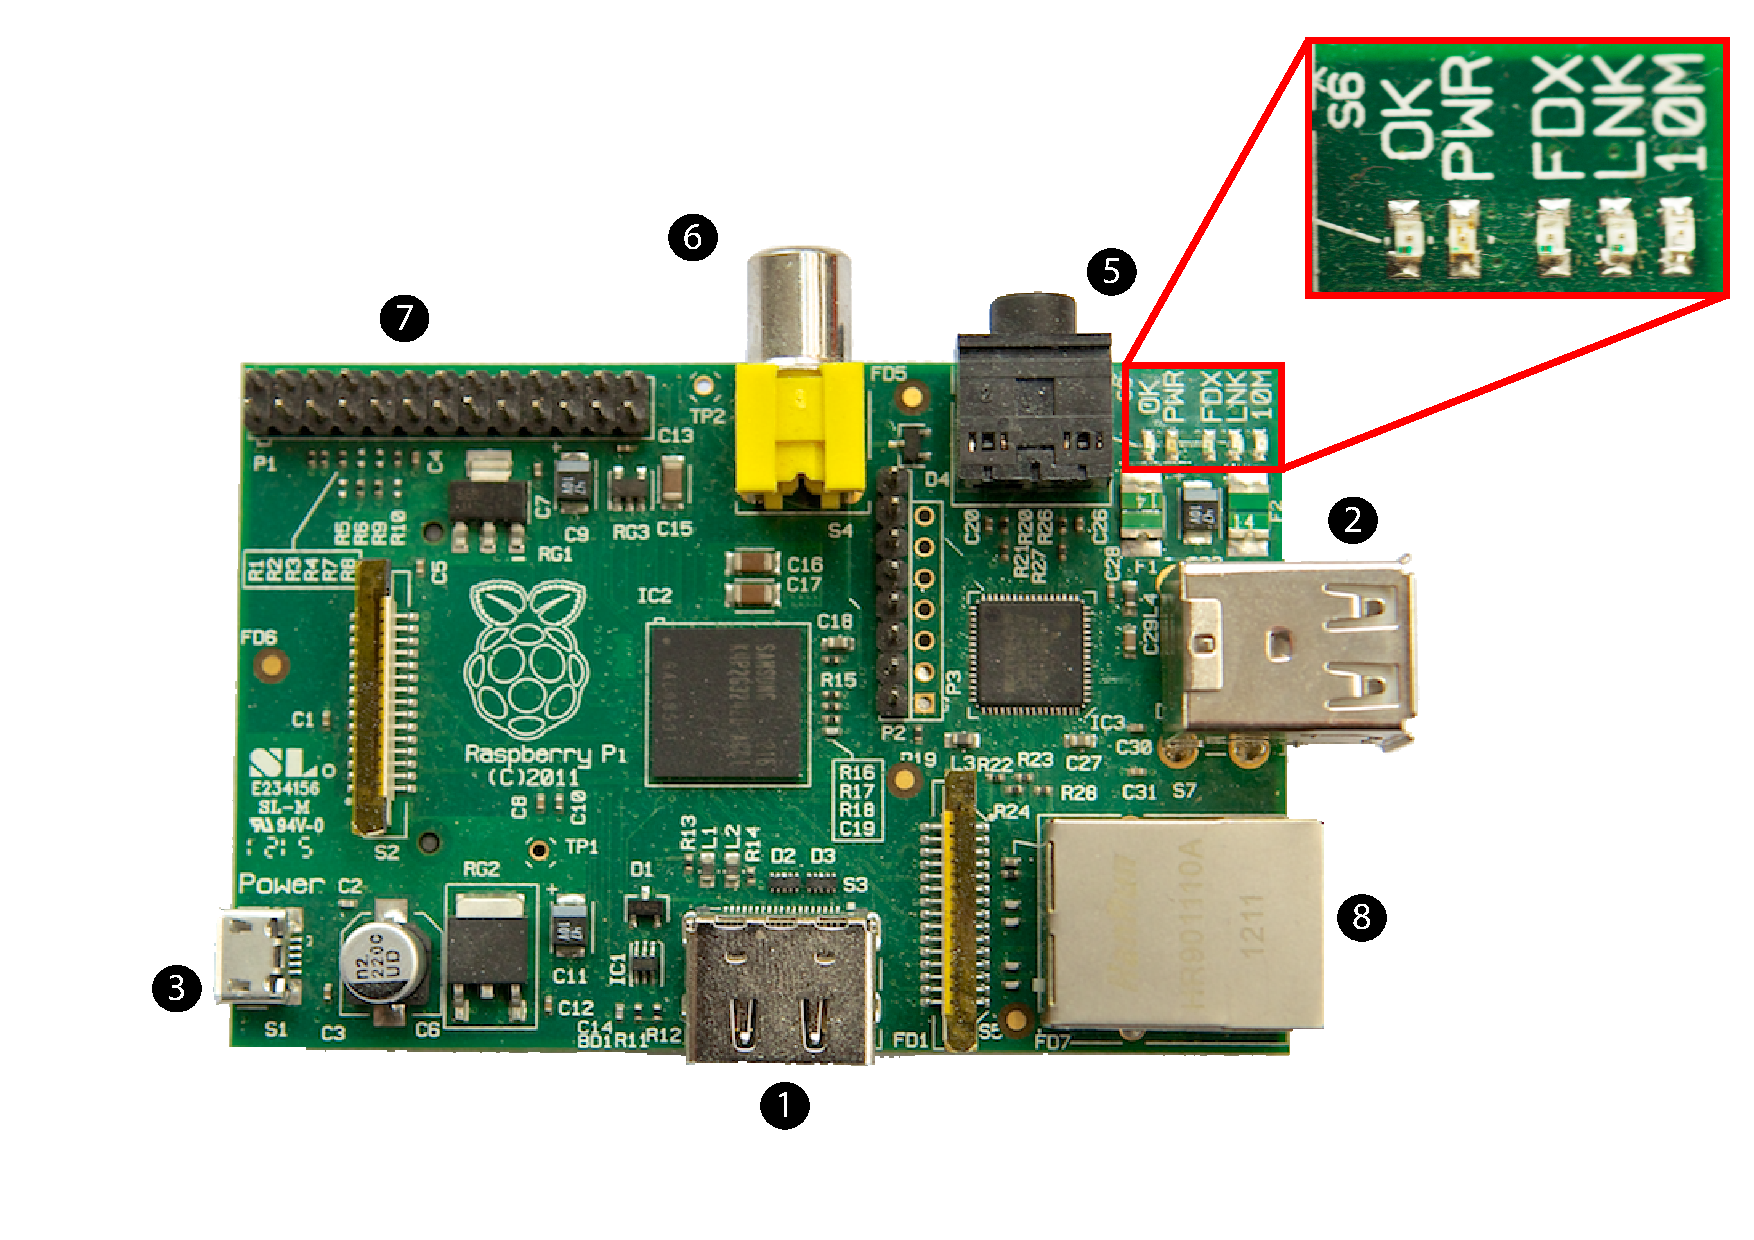
\includegraphics[width=15cm]{images/bare-rpi-annotated}}
\caption{An uncased Raspberry Pi, and an expanded view of the indicator LEDs at the board's top right. The numbered connectors are \protect\circled{1} HDMI output,  \protect\circled{2} USB,  \protect\circled{3} power,  \protect\circled{5} audio output,  \protect\circled{6} composite video out,  \protect\circled{7} General Purpose Input/Output (GPIO),  \protect\circled{8} Ethernet.}\label{figure:bare-rpi}
\end{figure}

\begin{figure}
\centerline{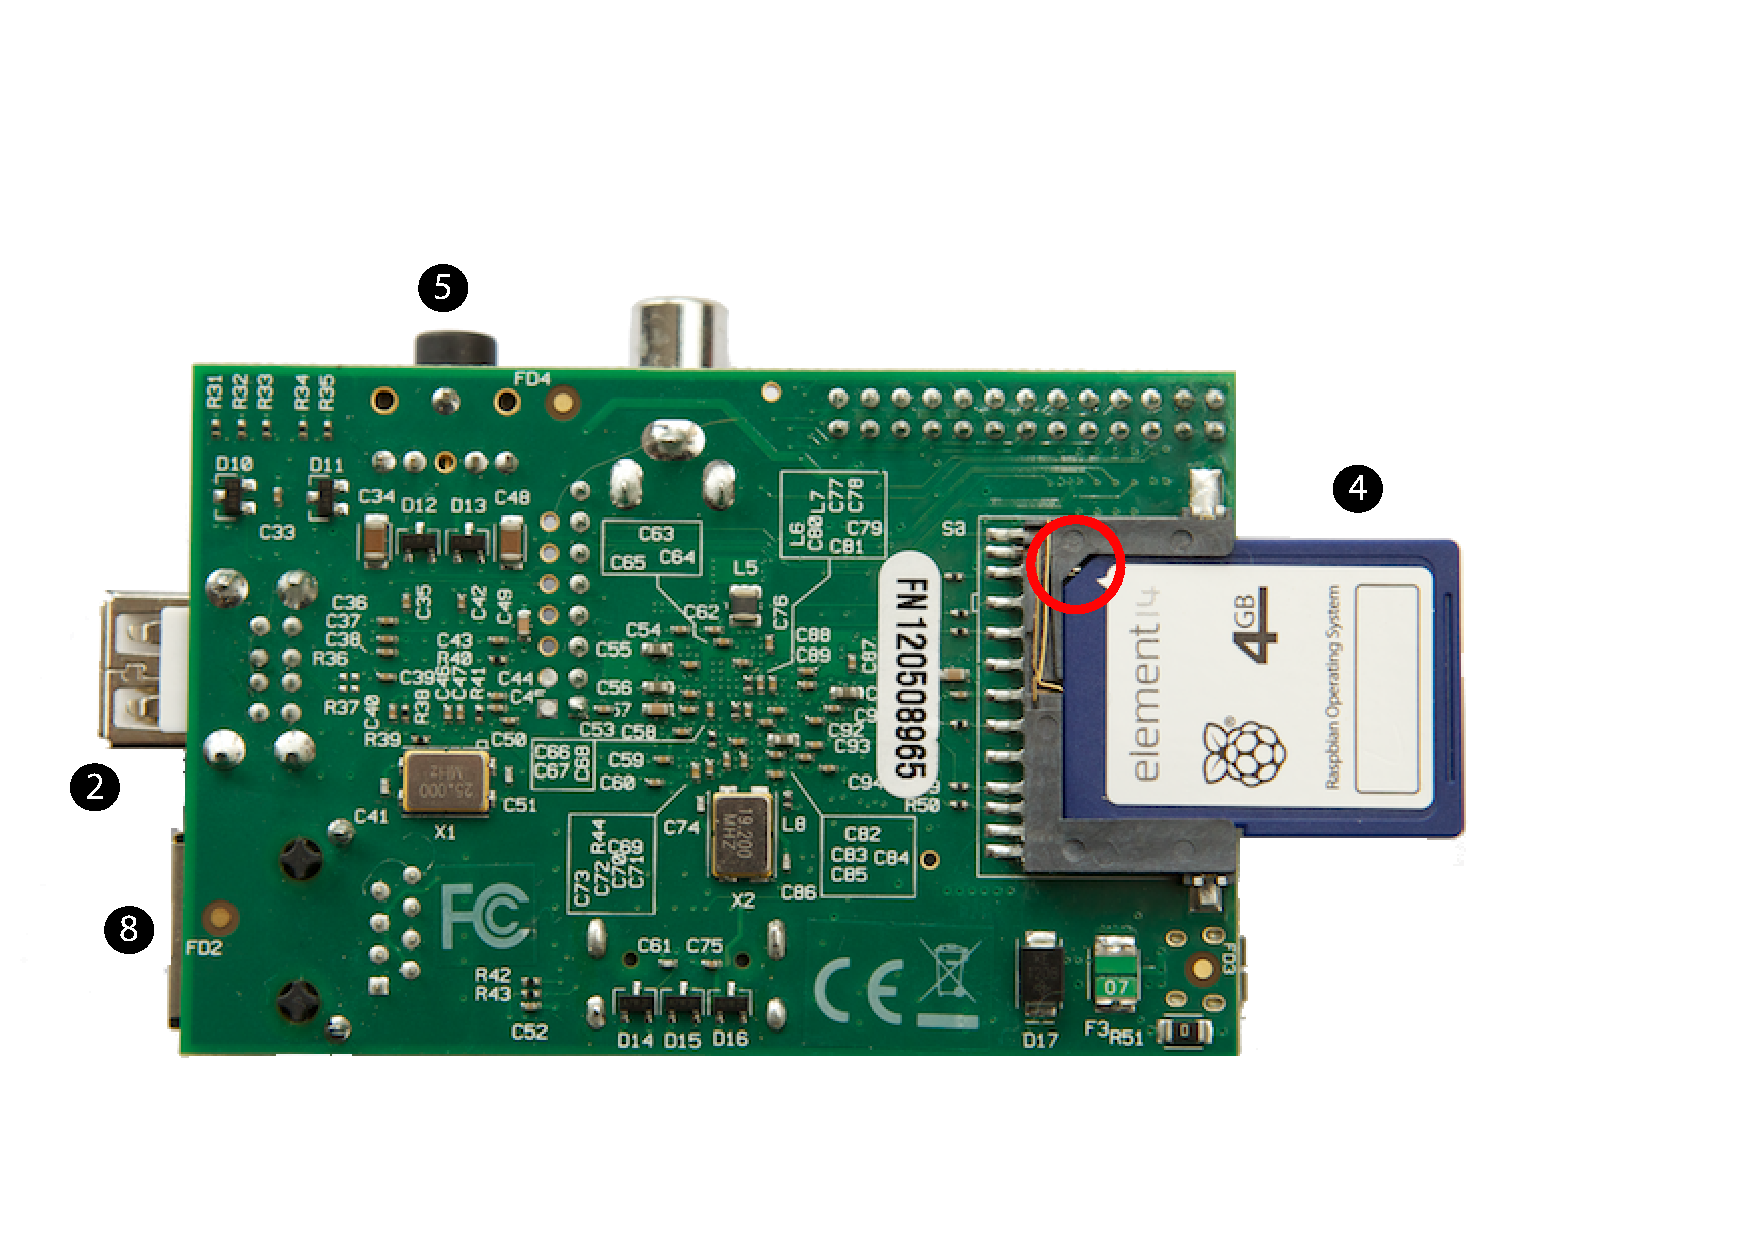
\includegraphics[width=15cm]{images/bare-rpi-underside-annotated}}
\caption{A naked Raspberry Pi. The circle indicates the location of the bevelled corner to orient the card. The ports are numbered as in Figure~\ref{figure:bare-rpi}, and in addition \protect\circled{4} shows the location of the SD (Secure Digital) memory card.  The locating bevel on the card is circled.}\label{figure:bare-rpi-underside}
\end{figure}

It's important that you connect the Pi up in exactly the order specified here---so even if you are familiar with using a Pi, please don't jump ahead and plug everything in at once (no harm will come to the Pi if you do, but this exercise relies on your following our instructions closely). Refer to Figure \ref{figure:cables}, and then connect your Pi up like this:

\begin{figure}
\centerline{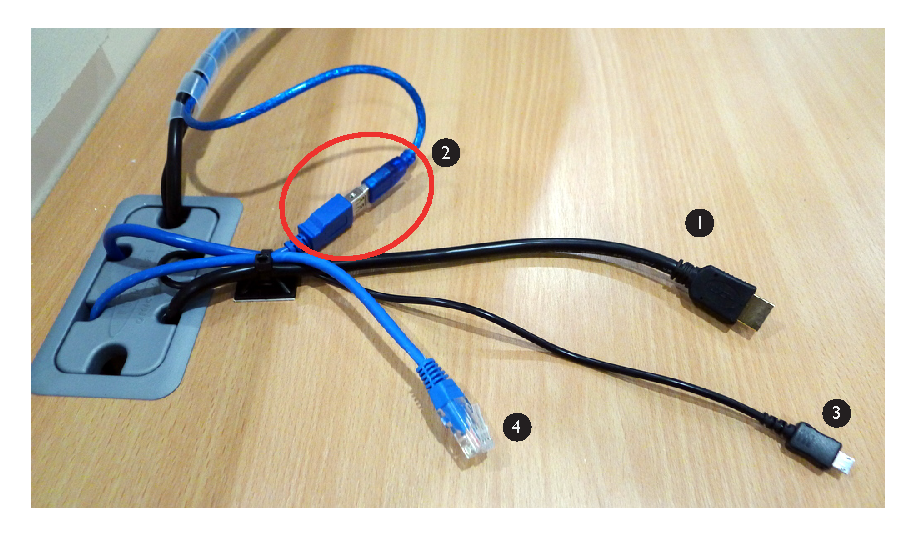
\includegraphics[width=13cm]{images/cables}}
\caption{The following cables are available to connect up your Pi. \protect\circled{1} HDMI, \protect\circled{2} Keyboard and Mouse, \protect\circled{3} 5 Volt Micro USB power supply, and \protect\circled{4} network.}\label{figure:cables}
\end{figure}


\begin{itemize}
\item The monitors in the LF31 Lab are all fitted with an extra video lead for connecting up the Pis. Locate the HDMI lead (labelled \protect\circled{1} in Figure \ref{figure:cables}), and plug this into the socket marked \circled{1} on Figure~\ref{figure:bare-rpi}. 
\item Next we'll need to connect a keyboard and mouse. Separate the male and female USB connectors marked \protect\circled{2} on Figure \ref{figure:cables}, and plug the male end into one of the two USB sockets on your Pi (marked with \protect\circled{2} on the Figure~\ref{figure:bare-rpi}). It doesn't matter which USB socket you choose, but please make sure to reconnect this to the PC when you're done with these experiments as a courtesy to the next user. 
\item \textbf{Do not connect the power or network connectors at this stage!}
\end{itemize}

Next, we need to insert the \wikipedia{Secure_Digital}{Secure Digital} (SD) card that contains the Pi's operating system, and on which you'll be storing your own files. Look at Figure ~\ref{figure:bare-rpi-underside}, make sure the SD card is orientated correctly (note the position of the little cut corner) and gently push it into the socket; around half of the card will remain protruding outside the case. 


Now you're ready to power up the Pi. In our lab setup in LF31 the power to the Pi is supplied via the monitor, so it is important that the monitor is not in standby mode. Standby is indicated by an orange light on the on/off button at the bottom right of the screen, rather than blue if it is on. If the light is orange, press it to turn the monitor off, then again to switch it back on and turn it blue. Now locate the 5v Micro USB cable (the same connector that you'll find on many modern smartphones and tablet devices); this is labelled \protect\circled{3} on Figure~\ref{figure:cables}. This goes into the socket marked \circled{3} on Figure \ref{figure:bare-rpi}. There is no power switch on the Pi, so as soon as the power cable goes in, it will start to boot (this strange term is explained in breakout box~\ref{bootbox}): the red PWR LED should light up and stay on, and you'll also notice that the OK LED (which indicates SD-card activity) to its left also flickers. If any of the other three LEDs marked FDX, LNK, or 10M are lit, then that means you've already plugged a network cable into your Pi, in which case please unplug that now!



% Moved this Danger Box to intro1 
%\begin{danger}{Pi Power} 
%Like most other computers, the Pi doesn't like having its power removed without being shut down properly. Although you might get away with it, there's a reasonable chance of messing up the operating system if you remove the power while the Pi is in the middle of doing something. And because the Pi runs a multi-tasking operating system, it's almost always `doing something', so pulling the power out unexpectedly is always a bad idea. You're unlikely to damage the Pi's hardware like this, but you may find that you lose work, and may have to reinstall the operating system. For instructions on how to shut the Pi down safely, see Section \ref{section:shutdown}.
%\end{danger}

Now we need to switch the input on the monitor from DisplayPort (which
is the input used by the PC under the desk) to DVI (the cable you've
connected your Pi to is a HDMI to DVI cable). On the lower-right side
of the monitor you will see 4 buttons -- see
Figure~\ref{figure:monitorswitch}. Press any of them to bring up the
monitor's menu. Now press the 3rd button down and navigate to the
input selection menu. Switch the Input to DVI and all being well you
should see a black screen containing the Raspberry Pi logo at the top
left, and white text that scrolls up the screen as the Pi boots.

\begin{figure}
\centerline{\includegraphics[width=12cm]{images/DellInputMenu.jpg}}
\caption{The Input Selection menu on the monitor. This image  of the Dell U2412M Monitor has been reproduced with the kind permission of Dell. All rights reserved.}\label{figure:monitorswitch}
\end{figure}

When the boot process finishes for the first time (it will take somewhere
about 20--30 seconds), if all has gone well you should see the NOOBS (New Out Of Box)
installation tool appear (see Figure \ref{figure:noobs-install-screen}).

\begin{figure}
\centerline{\includegraphics[width=13cm]{images/noobs-install-screen}}
\caption{NOOBS Install Screen}\label{figure:noobs-install-screen}
\end{figure}

\subsection{Installing Raspbian}

The SD card that comes with your Pi is set up so that when you first start the device you can choose to install one of a variety of different operating systems that are compatible with the Raspberry Pi hardware. We are going to use Raspbian for all of the labs, so scroll down the list until you see an option labelled Raspbian with an SD card icon to the right, and check the left hand box as shown in Figure \ref{figure:noobs-select-raspbian}. \emph{Take care not to select the other Raspbian option with a network connection icon, as this will attempt to download Raspbian over the network.}

\begin{figure}
\centerline{\includegraphics[width=13cm]{images/noobs-select-raspbian}}
\caption{Selecting Raspbian}\label{figure:noobs-select-raspbian}
\end{figure}

Click the Install button and you will see a final warning message as in Figure~\ref{figure:noobs-install-warning}. Click Yes to confirm, and the installation process shown in Figure \ref{figure:noobs-install-progress} will begin. This process will take around 15 minutes to complete, so while you're waiting for Figure~\ref{figure:raspi-config} to appear please use the time to read Section~\ref{sec:unix-linux} in the separate handout then come back here to complete the installation process.
\label{page:raspbian-install}
  
\begin{figure}
\centerline{\includegraphics[width=13cm]{images/noobs-install-warning}}
\caption{Final warning/confirmation from NOOBS}\label{figure:noobs-install-warning}
\end{figure}

\begin{figure}
\centerline{\includegraphics{images/noobs-install-progress}}
\caption{NOOBS installation progress}\label{figure:noobs-install-progress}
\end{figure}

\begin{rpi}{Raspbian}
  Raspbian is a version of the Debian release of Linux, tuned for the Pi. If you manage to corrupt the operating system, or just want to start from scratch, then re-writing the SD card with a fresh image is reasonably straightforward: simply reboot your Pi and press the Shift key when the initial splash screen loads (you will need to be quick, as it only appears for a few seconds). This will present you with a list of options. Ensure that Raspbian is selected and then click the Install icon to re-write the SD card with a fresh image. This will erase all of the data on the Pi, so it's crucial that you make sure that you have a backup of anything important.

  If you buy a new SD card, instructions on how to get hold of the files you'll need, and how to write them to the SD card on various operating systems are available at \urlnop{www.raspberrypi.org/downloads}. You might want to think about getting a larger SD card in any case; the one we've given you is fine for the labwork we've set, but probably a bit on the small side for anything else. SD cards are widely available in shops and online, and aren't expensive. But you should check whether the specific card you're going to buy is compatible with the Pi before parting with any money---differences in the read/write speeds of some cards mean they don't play nicely with the Pi.
\end{rpi}


\begin{diversion}{Booting}
\label{bootbox}
The phrase `booting' to refer to the process of starting up some computer system has become quite commonplace, but its origins are rather strange. It's thought to have first been used in early 19th Century America as a way of describing an obviously impossible action such as to ``pull oneself over a fence by one's bootstraps''. These days it is used to refer to any self-sustaining process that is able to happen without external help. 

So why is starting a computer a bootstrapping process? In order for you as a user to be able to run a program, the computer needs an operating system. But in order to load its operating system, it needs some instructions that tell it how to understand the file system. And in order to load the instructions that tell it how to understand the file system it needs to\ldots well, you get the idea. In reality, most computers have a very small set of instructions hardwired into them that begin the process of loading a  slightly more complex `bootloader', which then begins the process of loading the OS kernel and any modules needed to interact with the hardware, and then starts loading services and features of increasing sophistication that rely on the simpler ones loaded previously to function. 

As an aside, you may want to consider this: if you need a text editor to write programs, how did the first text editor (which is itself a program) get written?
\end{diversion}

\begin{figure}
\centerline{\includegraphics[width=13cm]{images/raspi-config.png}}
\caption{The Raspberry Pi config tool. The highlight bar can be moved between the different controls using the Tab key, or up and down in the menu using cursor keys.}\label{figure:raspi-config}
\end{figure}

Once Raspbian has finished installing, the Pi will reboot and you will
be presented with a configuration screen as shown in Figure \ref{figure:raspi-config}.
At this stage you could tweak various other options that affect the
display and the layout of keyboard being used; but conveniently the
defaults set on the Pi will do just fine for now (it is a mostly
British invention after all, so it defaults to UK keyboard layout!)
Use the Tab key to move the red highlight to \ttout{<Finish>}, and hit
Enter again.
% Confirm that the Pi should reboot (an example of what
% this looks like is shown in Figure \ref{figure:piboot}) and this time
% when the process finishes you'll be presented by a Unix login prompt
% which will say something like:

%\begin{figure}
%\centerline{\includegraphics[width=15cm]{images/bootscreen}}
%\caption{A sample Raspberry Pi bootscreen. The exact layout and details may vary depending on the size/shape of the screen and the configuration of the Pi.}\label{figure:piboot}
%\end{figure}

%\begin{ttoutenv}
%Debian GNU/Linux wheezy/sid raspberrypi tty1

%raspberrypi login:
%\end{ttoutenv}


%\subsection{Shutting down the Pi}
%\label{sec:shutting-down-pi}

%Like any other computer, its really important that you shut your Pi down properly; if you just pull the power cord out there's a chance of corrupting the filesystem. To shut the Pi down safely you first need to login using the username \ttout{pi} and the password \ttout{raspberry}. \textbf{Note that, so that anyone standing behind you cannot even see the length of your password,  the username will appear on screen as you type it, but the password will not}.
You will then see a screen which contains a prompt looking like

\begin{ttoutenv}
\textbf{pi@raspberrypi ~ \$  }
\end{ttoutenv}
on which you should type the command
% $

\begin{ttoutenv}
sudo halt
\end{ttoutenv}
followed by the Return key.

\noindent We'll explain a bit more about what's going on here in the next lab session, but for now please just follow the instructions.

%\noindent You'll see the a series of messages scroll past that look rather like those you saw during the boot process. This shouldn't be surprising, since what the operating system is doing now is shutting down all the things that it started up when you booted the machine, roughly in reverse order.

The  Pi will now power itself down; the network  and OK LEDs will go off, the screen should go black, and only the red PWD LED will remain lit on the circuit board. At this point it's safe to pull the Micro-USB cable out of the Pi. Please make sure you reconnect the USB connector for use with the PC  as a courtesy to the next user, \emph{taking care to connect the USB cable the correct way round. } Make sure that you leave the desktop PC booted into Linux.

That's all we want you to do with the Raspberry Pi for this session, we will start using it in earnest in the next session.  When you have completed the work for this session, please tell the lab supervisor so we know how you're getting on. Remember, if you don't finish it during the lab session, please try to do so before the next one.

\textbf{Please make sure you bring your Pi and this set of notes to all the introductory lab sessions.}

\cleardoublepage

\section{Unix and Linux}
\label{sec:unix-linux}


Over the next couple of weeks you will be undertaking a number of
introductory labs to familiarise yourself with the School's computing
infrastructure. Much of this is based on devices and machines running Linux, a
variant of the Unix family of operating systems; this document
provides some background on Unix and explains why we think it is
important. It would very useful if you could read this before you
attend the first introductory labs, where the emphasis will be on
leading you through a series of tasks to explore our setup.

\subsection{Operating Systems}

An \wikipedia{Operating_system}{operating system} (OS) is a suite of
software that makes computer hardware usable; it makes the `raw
computing power' of the hardware available to the user. You're
probably most familiar with
the \wikipedia{Microsoft_windows}{Microsoft Windows} and
Apple \wikipedia{OS_X}{OS X} families of operating systems for
`desktop' computers, and \wikipedia{Ios}{iOS} (Apple, again) and
Google's \wikipedia{Android_(operating_system)}{Android} for mobile
devices; but many other more specialist operating systems exist, and
you'll be studying some of these and the principles that underpin OS
design in COMP25111 in your second year. In the meantime, a potted
history of OS development will tide us over\ldots
 
\subsection{Unix Origins}
\label{sec:unix}

In the late 1950s, an American company
called \wikipedia{Bell_Labs}{Bell Laboratories} decided that they
needed a system to improve the way they worked with their computer
hardware (it's probably quite hard to imagine what interacting with a
computer \emph{without} an operating system might be; but it wasn't
pretty and involved manually loading and running programs one by
one). Together with the \wikipedia{General_Electric_Company}{General
Electric Company} and the \wikipedia{MIT}{Massachusetts Institute of
Technology}, they set about the design of an operating system they
called \wikipedia{Multics}{Multics}: the `Multiplexed Information and
Computing Service'. Multics was hugely innovative, and introduced many
concepts that we now take for granted in modern operating systems such
as the ability for more than one program to run `at once'; but it did
rather suffer from `design by committee', and the final system was
seen at the time as being overly complex and rather bloated (`bloated'
is all a matter of perspective of course: its sobering to realise
though that the entire Multics operating system was only around
135Kb. Today's operating systems are something like 30,000 times this
size\ldots). In the late 1960s, a group of programmers at Bell Labs
created a cut-down, leaner and cleaner version of Multics that would
work on more modest hardware. Legend has it that this was to allow
them to play their favourite (only!) computer
game, \wikipedia{Space_Travel_(video_game)}{Space Travel}. In an early
example of the trend of giving things `punny' names, to contrast with
the more clumsy Multics, they called this new system Unix. The
so-called \wikipedia{Jargon_File}{Jargon File} is a good source of
explanations of various bits of computer slang and their obscure
origins, and is well worth a read: in part to give some background
history, but mostly as an insight into the minds of the computing
pioneers of the past!

%\begin{htmlonly}
%(See the Unix entry in the useful and amusing
%\htmladdnormallink{Jargon
%file}{http://www.new.ox.ac.uk/admin/jargon/html/entry/Unix.html}, a
%file}{http://www.cs.manchester.ac.uk/software/jargon/html/entry/Unix.html}, a
%file}{\jargonFileUnix}, a
%`collection of slang terms used by various subcultures of computer
%\htmladdnormallink{hackers}
%{http://www.cs.manchester.ac.uk/software/jargon/html/entry/hacker.html}'.)
%{\jargonFileHackers}'.)
%\end{htmlonly}

Even though Unix is now quite old, most Computer Scientists recognise that the designers of Unix got most of the fundamental concepts and
architecture right. Given how much computing has changed since the 1960s, this was an astonishing intellectual achievement. Although Microsoft's \wikipedia{Microsoft_Windows}{Windows} is by far the most common operating system on \emph{desktop} machines, the majority of the Internet, much of the world's corporate infrastructure, virtually all supercomputers, and even some mobile devices are powered by Unix-like operating systems. So, while the polished graphical user interfaces of Windows and \wikipedia{OS_X}{OS X} appear to dominate the world of computing, most of the real hard-core and leading-edge computation relies on an elegant operating system designed nearly 50 years ago (by a team of scientists who wanted to play a game).  

\subsection{Modern Unix Variants}
\label{sec:modern-unix-variants}


The history of Unix is complex and convoluted, with the system being updated, re-implemented, and mimicked repeatedly over the years, primarily by commercial companies who guarded their versions jealously. Figure \ref{fig:unix-history} shows a tiny fragment of the Unix's `family tree' (the full diagram, which you can find at \urlnop{www.levenez.com/unix/unix.pdf}, is \emph{many} times the size of the portion you can see here).

\begin{figure}[h!tb]
  \begin{center}
    \includegraphics[width=13cm]{images/unix}
  \end{center}
\caption{A fragment of \'{E}ric L\'{e}v\'{e}nez's Unix History chart, reproduced with permission and showing the beginnings of Linux in amongst other versions of Unix.}
\label{fig:unix-history}
\end{figure}
 
Although many of the branches represent interesting innovations of one kind or another, there are perhaps two that deserve particular attention. The first of these was the decision by Apple some time around the turn of the millennium to drop their own---highly popular, but ageing---bespoke operating system (unimaginatively called \wikipedia{Mac_os_9}{Mac OS 9}) in favour of a Unix-based system (now the more familiar `OS X', where `X' is both the Roman numeral `10' and a nod in the direction of the uniX nature of the OS). Although the majority of Mac users are blissfully unaware of the fact, behind the slick front-end of OS X, sits a variant of Unix. The second, and perhaps more profound of these events was the creation in 1991 by Swedish programmer \wikipedia{Linus_torvalds}{Linus Torvalds} of a Unix-like system, the source code to which \emph{he gave away for free}\footnote{`free' here in the sense both of `freedom to reuse or adapt', and also in the sense of `without charge'.}; this became known as the \wikipedia{Linux_kernel}{Linux Kernel}. Combined with other free software created by the \wikipedia{Free_software_foundation}{Free Software Foundation}, a non-commercial version of Unix called \wikipedia{GNU/Linux}{GNU/Linux} was born (GNU here is a recursive acronym for ``GNU's not Unix'', a swipe at other commercial non-Free versions; much to the annoyance of the Free Software Foundation, GNU/Linux is almost always called just `Linux'\footnote{Linux
is pronounced ``Linn-ucks'', despite the fact the name was coined by
its creator, and his name `Linus' is pronounced
``Leen-uss''!}.) 

Linux has been, and continues to be, developed cooperatively by
thousands of programmers across the world contributing their effort
largely free of charge. It is amazing to think that such
a project could ever happen---and it is surely a testament to the
better side of Human Nature. But what is interesting is the
observation that these programmers are not motivated by commercial
concerns, but by the desire to make good reliable software and have it
used by lots of people. Thus, Linux is a good choice of Unix: it's
Free, it's efficient, and it's reliable, and it is now used by large corporations, governments, research labs and individuals around the world. Even Google's \wikipedia{Android_(operating_system)}{Android} platform is a Linux-based mobile OS, and the  \wikipedia{Amazon_Kindle}{Amazon Kindle} is also a Linux box behind the electronic ink of its user interface (Figure \ref{fig:kindlelinux}).

\begin{figure}[h!tb]
  \begin{center}
    \includegraphics[width=13cm]{images/kindleroot}
  \end{center}
\caption{A photograph of Liraz Siri's `rooted' kindle, showing the Linux command prompt. Reproduced with the author's kind permission from \urlnop{www.turnkeylinux.org/blog/kindle-root}}
\label{fig:kindlelinux}
\end{figure}

One of the results of the fact that Linux is Free is that several
organisations and companies have created their own distributions of
it; these vary a bit (in fact, anybody is free to make any change they
like to Linux, and pass it on to whoever wants it). The distribution
we use in this School is \textbf{Scientific Linux}, which is
based on a distribution by a
US company called \textbf{Red Hat}.
%, which is the latest release

So, if you are to become an expert computer professional, it is
important that you understand the theory and practice of Unix based
systems. Learning Unix is not only a crucial skill for any serious
computer scientist, it is a very rewarding experience; the labs over
the next couple of weeks are designed to help you become familiar with what will be your daily working environment.

If you haven't done so already, please return to Section~\ref{page:raspbian-install} on page~\pageref{page:raspbian-install} to complete the Raspbian installation. When you have completed the work for this session, please tell the lab supervisor, so we know how you're getting on.

\textbf{Please make sure you bring your Pi and this set of notes to all the introductory lab sessions.}

\renewcommand{\chaptername}{Intro Lab Session}
\coursecode{Introductory Labs}
\include{intro1}
\chapter{Using the Linux desktop in CS}

\minitoc

\notesurl{intro2}

\begin{demonote}
  Part of this lab involves editing dot files. Any mistake here can result in a student not being able to login. To fix this, login yourself (either on a new virtual terminal or another machine), then
  \begin{ttoutenv}
    cd /tmp
    su [studentloginname]  ## \textbf{Note not su -}
    cd \textasciitilde
  \end{ttoutenv}
  You can then poke around the dot files and fix the problem. Often this involves removing, or just renaming, the offending dot file

\end{demonote}
 Today we're going to explore some of the features of Unix in a bit more depth, this time using the desktop PCs rather than your Raspberry Pi (we'll return to using that in the next lab). We'll explore some of the more advanced features of the command line and various useful tools that will help you understand how a typical Unix system is organised. Almost everything that you learn using Linux on the desktop machine is equally applicable to the Raspberry Pi, and vice versa. 

\section{Logging in}

%%% BEGIN CONSOLE MODE SESSION
 Make sure the desktop PC is booted into Linux, and log in using your University username and password (\emph{not} the username and password you used on the Pi). Remember that nothing will appear on the screen when you type your password. You should be greeted with a similar, but rather longer, command prompt to the one you saw in the previous lab.

You are now logged in to a PC that is part of our School Linux network. Type \cmnd{pwd}{pwd} to find out which directory you are in. It should be something like \ttout{/home/mbaXXXXX}, where the part after the \ttout{/} is your username. This is your home directory which is not actually stored on the desktop PC but on a central fileserver. This means that, whichever machine you use in the lab, you will always see the same home filestore. Later we will be using a graphical environment, but for now we will stick to the console and start off by reading mail.


\section{Reading email at the console}

You're probably familiar with reading email using either a web-based interface, a graphical desktop application (such as Outlook, Thunderbird or OS X Mail) or using an app on a smartphone or tablet. Today you're going to do something slightly different, and configure a text-based mail client so that you can read your University email while at a console. The email client we're going to use is called \cmnd{mutt}{Mutt}, which is fairly simple to configure and straightforward to use (according to its author, Michael Elkins, ``All mail clients suck. This one just sucks less''). There are plenty of other similarly lean text-based \wikipedia{List_of_email_clients}{email clients}, and you may at some point want to check out \ttout{Alpine} as a sensible alternative to \cmnd{mutt}{Mutt} or for the historically-curious, \ttout{Elm} (if you want a \textit{really} hardcore console-mode experience of mail, look up \wikipedia{Mailx}{Mailx}).

First, let's confirm that \cmnd{mutt}{Mutt} is actually installed. 

To see if \cmnd{mutt}{Mutt} is installed and is accessible to you, use the \cmnd{which}{which} command. Type

\begin{ttoutenv}
\$ which mutt
\end{ttoutenv}

This should respond with \fname{/usr/bin/mutt}, telling us that the \fname{mutt} command has been put in the \fname{/usr/bin} directory on our system. Remember in the last sessions we looked at the contents of the \fname{/bin} directory that contained essential low-level commands such as \ttout{ls}? Well \fname{/usr/bin} contains commands that aren't quite as essential, but have been installed for the users' benefit (i.e. the system would boot and work without them, but it just wouldn't be very useful.) 

List the contents of \fname{/usr/bin} by typing
\begin{ttoutenv}
\$ ls /usr/bin
\end{ttoutenv}

and notice that here we're using \cmnd{ls}{ls} to look at the contents of a directory other than the one we're currently in by passing the directory name as a argument. A whole load of things should scroll past on the screen; most of them won't mean anything to you right now, but don't worry, we'll look at some of the important ones soon enough. Now that's a lot of stuff to look through, and depending on the size of your screen the command we're looking for may have scrolled off the top. So let's try to narrow our results down a bit. Type 

\begin{ttoutenv}
\$ ls /usr/bin/ma*
\end{ttoutenv}


and you should be given a much smaller list of things from the \fname{/usr/bin} directory; only those starting with the letters \ttout{ma}. The asterisk symbol is interpreted as being a `wildcard' that stands for `anything of any length, including length zero', so the command you've just typed means `list the contents of the \fname{/usr/bin} directory, showing only files that start with the letters \ttout{ma} and then are followed by zero or more other characters' (notice that the \ttout{man} command that you used in the last session is there amongst the results). 

You could narrow this down even further by typing \ttout{ls /usr/bin/man*}, in which case you'll only get files from \fname{/usr/bin} that start with the letters \ttout{man}. Note that if you leave off the asterisk from your command, you'll be asking for files that are called \textit{exactly} \ttout{ma} or \ttout{man}, which isn't what you want here.

So far we've been getting you to do a fair amount of typing, and now we have to admit that you've been typing a lot more than you actually need to (it's good practice though, so we're not feeling too guilty at this stage). The default Linux command line has a feature similar to autocomplete that you'll have seen on web forms and in graphical tools, that saves you typing full commands by suggesting possible alternatives. 

Type \ttout{ls /} but don't hit Enter, and instead press the Tab key twice. You'll be shown a list of sensible things that could follow what you've typed---in this case it's the list of directories that are in the system's root directory. Now type the letter \ttout{u} (so that the line you've typed so far should read \ttout{ls /u}) and hit Tab once. This time your command will be expanded automatically to \ttout{ls /usr/} since that's the only possible option. Press Tab twice now, and you'll get shown the contents of \fname{/usr/}. Type \ttout{b}, and press Tab to expand the command to \fname{/usr/bin/}, and then press Enter to execute the command.

The \wikipedia{Autocomplete}{autocomplete} function you're using here is more commonly called \concept{tab complete} by Unix users. If you press Tab once and there's exactly one possible option that would autocomplete what you've typed so far, then that option gets selected; if there are multiple possible things that could complete your command, then Tab will complete as far as it it can, then pressing Tab a second time shows you all of them, giving you the option to type another character or two to narrow down the list. Learning to use this will save you a lot of typing, because not only does it reduce the number of characters you type, it also helps you browse the options/files at the same time. 

% \begin{note}
% Need to work out how to explain tab complete for single things that have the same prefix
% \end{note}


Here are some other very useful command line tricks:

\begin{itemize}
\item You can use the up and down arrow keys to cycle back and forth through the list of commands you've typed previously.
\item The left and right arrows do what you expect, and move the insertion point back and forth. Pressing \ctrl{a} will move you to the start of the line, and \ctrl{e} to the end of the line (much faster than moving backwards and forwards character-by-character). 
\item \ctrl{c} aborts the current line, so if you've typed a line of gibberish, don't waste time deleting it one character at at time, just \ctrl{c} it!
\item Typing \ttout{history} lists all the commands you've typed in the recent past, useful if you've forgotten something.
\item Pressing \ctrl{r} allows you to retrieve a command from your history by typing part of the line (e.g. if you searched for `\ttout{whi}' now, it'll probably find the `\ttout{which mutt}' line you typed a while back). Pressing \ctrl{r} again cycles through possible matches (if more than one)
\item Pressing \ctrl{t} swaps the two characters before your cursor around. What, really? Yes: you'll be surprised how often you type characters in the wrong order! 
\end{itemize}

Back to configuring your email client. Before we use \cmnd{mutt}{mutt}, we need to point it at the incoming and outgoing email servers, and we'll do this by creating a configuration file.

\begin{diversion}{File extensions}
\label{diversion:file-extensions}
If you've mostly used Windows or OS X via a GUI, then you're probably used to files such as \fname{cheese.jpg}, where you would interpret \fname{cheese} as being the file \textit{name} and \textit{jpg} as being the file \textit{extension}. Some operating systems---notably Windows---have the notion of a \wikipedia{Filename_extension}{filename extension} of a particular number of characters built in; for example things ending with \fname{exe}, \fname{bat} or \fname{com} mean that they are executable files. In Unix, a file extension is merely a convention that's not enforced or meaningful to the operating system. So although it's common to give files a suffix that makes it easy for a human to guess what kind of file it is, Unix itself just treats these as part of the file name. In fact, you can have multiple `file extensions' in a name, to indicate a nesting of file types. In the previous lab the file \fname{quake3.tar.gz} is a \concept{tar} archive that has been \concept{gzipped}, but the presence of the \fname{.tar} and \fname{.gz} parts are really just there to tell the user how to treat the file.
\end{diversion}

We've created a template file for you to get going with. Make sure you are in your home directory, then use the \ttout{curl} command as in the last lab session to fetch the template from  \\
\urlnop{studentnet.cs.manchester.ac.uk/ugt/COMP10120/files/mutt-template}


Remember, you're going to need to use a switch argument to tell \cmnd{curl}{curl} what it should call the file it's fetched: call it anything you like, but \fname{mutt-template} is a perfectly good name (if you're feeling uncomfortable about a file that doesn't have a file-extension, see Breakout~\ref{diversion:file-extensions} for more information). Let's look at the file to see what's in it. Type

\begin{ttoutenv}
\$ less mutt-template
\end{ttoutenv}


and you should see the following written to the screen:
\begin{ttoutenv}
\input{files/muttrc}
\end{ttoutenv}

% \begin{note}
% SORT IMAP SETTINGS, maybe use a shell pattern
% \end{note}

The \cmnd{less}{less} command is used to display textual content from files and other sources (if you want to know why it has such an odd name, look at Breakout \ref{diversion:less}). One of \cmnd{less}{less's} features is that it `pages' through text, so that if the file you are looking at won't fit on one screen, pressing the space key will move you on to the next `page'; you may notice that the \cmnd{man}{man} command you used in the previous lab session actually used \cmnd{less}{less} to display the manual pages.

\begin{linux}{Spaced out filenames}
Because of its roots in the early days of computing long before the advent of graphical user interfaces, Unix filenames tend not to have spaces in them because this conflicts with the use of a space to separate out commands and their arguments. The Unix filesystem does allow spaces in filenames, but you'll have to use a technique called `escaping' if you want to manipulate them from the command line; this involves prefixing spaces in filenames with the backslash character \textbackslash{} to tell the command line not to interpret what follows the space as a new argument. For example, a file called \fname{my diary.txt} would be typed as \fname{my\textbackslash{} diary.txt}. It's a bit ugly, but it works fine. 
\end{linux} 

\begin{diversion}{Less is more}
\label{diversion:less}
As we've mentioned before, many of Unix's commands are plays on words, puns, or jokes that seemed funny to the command's creator at the time. Though this gives Unix a rich historical background, it does rather obscure the purpose of some commands. A prime example of this is the \cmnd{less}{less} command, used to page through text files that are too large to fit on a single screen without scrolling. 

Early versions of Unix included a command called \cmnd{more}{more}, written by Daniel Halbert from University of California, Berkeley in 1978, which would display a page's worth of text before prompting the user to press the space bar in order to see \textit{more} of the file. A more sophisticated paging tool, called \texttt{less} on the jokey premise that `less is more' was written by Mark Nudelman in the mid 1980s, and has since replaced \texttt{more} in most Unix systems, including Linux. 
\end{diversion}

Don't worry too much about the details of this file for now. If you're already familiar with how IMAP and SMTP work together to provide your email service, then you'll be able to see what the contents of this template mean; if you're not, don't worry, it'll all be explained in detail in the \courseunit{COMP18112} (Fundamentals of Distributed Systems) course in the second semester. For now, we just need to edit that file to contain your details rather than the fake ones in the template you've just downloaded. But let's play it safe: rather than editing the actual file you downloaded, just in case you make a mistake, let's first make a copy of the file in your home directory. 


Quit less (using the same technique you used to quit the \cmnd{man}{man} command in the last lab session), and then enter

\begin{ttoutenv}
\$ cp mutt-template my-mutt-template
\end{ttoutenv}

Did you type all of that? If so, you've wasted several precious key presses! You could have typed \ttout{cp mu}, and then pressed Tab to expand it to \ttout{cp mutt-template}, and then added on the \ttout{my-mutt-template} bit yourself. It's a good habit to get into and will save you a lot of time over the next few years.

The basic form of the \ttout{cp} command takes two arguments, the first being the file you want to copy, and the second being the name of the file that will be created. Confirm that there is indeed a new file in your home directory using \ttout{ls}, and that its contents are what you expect using \ttout{less} (how would you find out what else the \ttout{cp} command could do?). 

To modify the file, you'll need to use a text editor. Type 
\begin{ttoutenv}
\$ nano my-mutt-template
\end{ttoutenv}

to invoke the \ttout{nano} editor. Although fairly basic, the nano editor has all the features you'll need to make these changes, and helpfully shows you the various keyboard shortcuts to do particular things such as saving and quitting at the bottom of the screen (remember, the caret symbol (\texttt{\textasciicircum}) is shorthand for `\ttout{ctrl}', so \texttt{\textasciicircum X} means '\ctrl{X}').

Now use it to make the following changes:

\begin{itemize}
\item Edit the line that starts \ttout{set my\_user\_name} to include your University email address.
\item Edit the line that starts \ttout{set my\_imap\_server\_name} to include the server name that you obtained from the Outlook client in My Manchester, it's probably something like \ttout{pod51002}.
\item Edit the line that starts \ttout{set realname} to include your real name, in whatever way you want it to appear in outgoing emails. Please use your proper name here and not a funny nickname.
\end{itemize}

When you've made the changes, write out the file to your filestore and quit back to the command line. Then use \cmnd{less}{less} to confirm that the file now looks exactly as you want it to. 

Now, \ttout{mutt} expects the file containing its configuration information to have a particular name, and that's not \ttout{my-mutt-template}, so we'll need to do something about that. The Unix \cmnd{mv}{mv} command is used to rename files or directories (it's short for `move'), so use that to change the name of the file to \fname{.muttrc} by typing, not forgetting the dot at the start of the second filename

% \begin{note}
% can we do something here to explain why mv is called mv?
% \end{note}

\begin{ttoutenv}
\$ mv my-mutt-template .muttrc
\end{ttoutenv}


\ttout{mv} may seem like an odd name for a command that is used to rename a file, but it actually has a number of uses, including moving a file from one part of the file hierarchy to another. You'll see more examples of this in a later lab session.

Rather like \cmnd{cp}{cp}, \cmnd{mv}{mv} takes two arguments; but instead of making a copy of the file, \cmnd{mv}{mv} just changes the name of the file given as the first argument to that of the second. 

Type \ttout{ls} to confirm that the file name has changed as you'd expect. 

Oh. But it's gone! Actually, no, it's still there, but it's just hidden! There's a Unix convention that filenames  starting with a full-stop symbol don't appear when you type \ttout{ls} in its basic form, because these are normally configuration files that you don't need to see on a day to day basis (the `\concept{rc}' part of the \fname{.muttrc} name stands for \concept{resource configuration}, another Unix convention). So to see these files you'll need to add an extra switch argument to \cmnd{ls}{ls}. Use the \cmnd{man}{man} command to find out what this switch is, and then use the switch to confirm that the \fname{.muttrc} file does indeed exist. 

Using this switch on \cmnd{ls}{ls} will reveal several other so-called \concept{dotfiles} that have been lurking in your home directory all along.
%Use \cmnd{less}{less} to look at the contents of the one called \fname{.bash\_history} and it should become obvious how the \ttout{history} command, and the `reverse search' function you used earlier work.

If you're confident that you now have a file called \fname{.muttrc} containing the correct configuration, you can now type \ttout{mutt} to start the program. 

It should be reasonably clear how you use \cmnd{mutt}{mutt} to send and receive email; if you get stuck there are plenty of online tutorials to help you out. Send yourself a test email to make sure that everything is working, and when you're confident you've mastered the basics of sending and reading using this tool, quit \cmnd{mutt}{mutt} to get back to the command line. One thing you should note is that \cmnd{mutt}{mutt} doesn't have its own editor for composing emails, so will use \ttout{nano} unless you change this to something else in the \fname{.muttrc} file. 

\section{Browsing the Web}

Although you will have experienced The Web so far as a highly graphical system, the technology that underpins it is for the most part text-based, and it is (just about!) possible to browse web pages using a console-mode application. It might seem like an odd thing to do, but there's an important point to be made here, so bear with us.

%and install the \cmnd{lynx}{lynx} package using \ttout{apt-get} (remembering you'll need also to use \ttout{sudo} to get root %privileges). 

%Once the package is installed

Try browsing the School's web pages using \cmnd{lynx}{lynx} by typing

\begin{ttoutenv}
\$ lynx http://studentnet.cs.manchester.ac.uk
\end{ttoutenv}

Rather like \cmnd{mutt}{mutt}, the \cmnd{lynx}{lynx} program has just about enough on-screen help for you to be able to browse around a little without any additional instructions from us.  You may find that when you follow some links, nothing very much appears to have happened; but scroll further down the page and you'll see the content that you're looking for.

You'll probably find using \cmnd{lynx}{lynx} an unsatisfying experience: tolerable, and probably okay in an emergency, but not how you'd ideally like to browse the web. And you might be wondering why we've even bothered to get you to try viewing the web through a text-only interface. Apart from the absence of images and videos etc., the main difference between using something like \cmnd{lynx}{lynx} and a regular browser such as Chrome, Firefox, Safari or Internet Explorer, is that you'll notice that web pages have been made into much more linear affairs than when they are rendered in a graphical environment. While you might expect to see the navigation links neatly arranged on the left or top of the page with the main content prominently displayed in the centre, seen through a purely textual interface it's all one big stream of stuff, and its very hard to distinguish between the navigation links and the main content. 

Now consider what the web `looks' like if you are visually impaired or blind and have to use a screen-reader (a voice-synthesiser program that vocalises the text that's on-screen) to interact with your computer. Whereas a sighted person can easily cope with a two-dimensional layout that allows you to be aware of multiple things at the same time (i.e. you can be reading the main content of the page, but conscious of the fact that there's a navigation bar on the left for when you need it), if instead you are listening to a voice reading the contents of the page out to you, it's only possible to be hearing one thing at a time. And what's more, you have to remember what has been read out in the past in order to make sense of what you are hearing now; you can't just `flick back' a paragraph or two by moving your eyes, instead you have to instruct the screen reader to backtrack and re-read something. So the experience of using the web if you are visually impaired has some things in common to interacting with web-pages using \cmnd{lynx}{lynx}. 

You'll soon be designing your own web-based systems as part of the Group Project in \courseunit{COMP10120}; making them accessible to visually impaired readers is something you should keep in mind. Try using \cmnd{lynx}{lynx} to browse some of your favourite websites, and you'll almost certainly find that the level of `accessibility' on the Web varies considerably!

\subsection{Pipes and Redirects}
\label{section:pipesandredirects}

One of the fundamental philosophies of Unix---and one that is a sensible philosophy when you're building any computer system really---is that the operating system is composed from lots of simple sub-systems, each of which performs one clearly defined task. To do something more complex than any of the individual tools allows you to do on its own, you are expected to combine components yourself. At the command line, Unix makes this quite simple, so let's give it a go. 

First, use lynx to look at the BBC's weather page at \urlnop{www.bbc.co.uk/weather} and have a quick browse around to get familiar with what it looks like. Then quit \cmnd{lynx}{lynx} and get back to the command prompt before typing:

Type:
\begin{ttoutenv}
\$ lynx -dump http://www.bbc.co.uk/weather
\end{ttoutenv}

Note the addition of the \ttout{-dump} argument before the URL this time. Instead of running as an interactive browser, \cmnd{lynx}{lynx} should have just output the text that it would have displayed for that page to the console, and then quit. Now, most of the text of the page will have scrolled off the top of the screen, so let's use the \ttout{less} command to allow us to page through \cmnd{lynx}{lynx}'s output in a more controlled manner. Type:

\begin{ttoutenv}
\$ lynx -dump http://www.bbc.co.uk/weather | less
\end{ttoutenv}

Did you type all that? Hopefully not---remember you can use the up and down arrow keys to get previous commands back at the interactive prompt, and then just modify or extend them to save wearing out your fingers.

To explain what's happened here, you'll have to understand the concepts of \concept{standard in} and \concept{standard out}, which are a neat and extremely powerful idea that is fundamental to the way tools (and programmes generally) work in a Unix environment. 

Every Unix program has access to a number of ways of communicating with other parts of the operating system. One, \concept{standard in} allows a stream of data to be read by the program; another, called \concept{standard out} gives the program a way of displaying textual responses. By default, when you execute things at the command prompt, the shell arranges for a program's standard in to be connected to whatever you type at the keyboard, and for its standard out to be connected to whatever display you're using at the time (this is a bit of an over simplification, but it'll do for now). It's quite easy to arrange for standard in and standard out to be connected up differently though, and that's what you've just done.

The vertical bar `\verb-|-' before \cmnd{less}{less} is called the \concept{pipe} symbol, and it is used to join the output of one command to the input of another; so in this case we have connected the standard output from \cmnd{lynx}{lynx} directly to the standard input of \cmnd{less}{less}. When \cmnd{less}{less} is invoked without a filename argument, it expects to get its input from standard in.

Instead of joining commands together, you can use the idea of manipulating standard in/out to create or consume files instead. Try:

\begin{ttoutenv}
\$ lynx -dump http://www.bbc.co.uk/weather > weather.txt
\end{ttoutenv}

and then use \ttout{ls} to confirm that a file called \ttout{weather.txt} has been created, and use \ttout{less} to look at its contents (which should be just the text from the weather web-page we've been looking at already). Here the \verb-`>'- symbol \concept{redirects} the standard out of the \cmnd{lynx}{lynx} command so that instead of going to the console display it gets put into a named file. 

To finish off this first contact with pipes and redirects, we'll use a new command called \ttout{grep} along with lynx to create a simple command of our own that tells you what the weather is like in Manchester (there are very few labs with windows onto the outside world in the Kilburn Building, so this may be more useful than you think!) 

\ttout{grep} is a hugely powerful and useful utility, designed for searching through plain-text files. Learning to master grep will take more time than we have in this lab, since you'll have to understand the idea of \concept{regular expressions} to make full use of it (we'll come to those in a later lab). For now, we'll use it in its very simplest form. Type:

\begin{ttoutenv}
\$ grep BBC weather.txt
\end{ttoutenv}

and you should see a list of all the lines from \ttout{weather.txt} that contain the word `BBC'. Use \cmnd{less}{less} to have a look for other terms to `\ttout{grep}' for (you might want to try something like `Sunny' to give you a list of all the places where the weather is nice, for example). 

Rather like \cmnd{less}{less}, if \cmnd{grep}{grep} isn't given the name of a file as its last command-line argument (in this case we used \fname{weather.txt}), it will operate on standard-input instead of grepping through a file (yes, it's quite okay to use grep as a verb from now, no one will look at you funny). Use this knowledge to join together \cmnd{lynx}{lynx} and \cmnd{grep}{grep} so that the output is a single line describing the weather in Manchester right now. The output should look something like:

\begin{ttoutenv}
   [33]Manchester 22\textdegree{}C 72\textdegree{}F
\end{ttoutenv}

As a final flourish, let's create a new a way of accessing this new `weather in Manchester' tool that you've created. Type:

\begin{ttoutenv}
\$ alias mankyweather="[YOUR COMMAND GOES HERE]"
\end{ttoutenv}

replacing [YOUR COMMAND GOES HERE] with the full command line you created to display the Manchester weather, being careful not to introduce extra spaces around \ttout{=}. Then try typing

\begin{ttoutenv}
\$ mankyweather
\end{ttoutenv}


to see the result. Okay, so this probably won't replace your favourite weather web page or app, but its early days yet! 
Note that this alias will disappear once you exit the shell in which you created this, for example when you logout and login again. We will see in a later lab how to make such aliases permanent.

%%% END CONSOLE MODE SESSION

\section{X Windows and GNOME} 

Next you're going to start up one of Linux's many graphical user interfaces. Type:

\begin{ttoutenv}
\$ startx
\end{ttoutenv}


You'll see a chunk of text scroll up the screen briefly before being presented with something that looks like the screen shot in Figure \ref{figure:gnome-desktop}.

\begin{figure}[t]
\centerline{\includegraphics[width=16cm]{images/gnome-desktop}}
\caption{Scientific Linux's default graphical user interface and
  window manager, GNOME 2. \protect\circled{1} the top panel contains
  a menu of applications and system controls, as well as shortcuts to
  some frequently-used tools. You can easily configure the shortcuts
  to include your favourite things. \protect\circled{2} a graphical
  file-browser called `Nautilus' gives you graphical access to your
  files much like Explorer on Windows or Finder on
  OSX. \protect\circled{3} Clicking on your name shows the `log out'
  option. \protect\circled{4} The `wastebasket' and virtual desktop
  controls}\label{figure:gnome-desktop}
\end{figure}

Take a few minutes to explore the graphical environment. Even if you've never used Linux before, you'll probably find the general principles of this environment quite familiar: there are icons on the desktop giving you access to the computer via a graphical file browser, and at the top of the screen a menu-bar allows you to start various applications and utilities. The full manual for this environment---which is called GNOME 2---is available online at 

\noindent\urlnop{personal.us.es/rledesma/descargas/gnome2.6-user-guide.pdf}

\begin{linux}{GNOME and Metacity}
It's quite common to refer to GNOME as a `window manager', but technically it is much more than that; it's actually a collection of tools, applications and other programs that together form a graphical desktop environment. The window manager component of GNOME 2 is called \wikipedia{Metacity}{metacity}.
\end{linux} 

\noindent but you'll probably be able to work out everything you need to get you going by poking around at the various buttons. Unlike the Raspberry Pi where you have complete control over the operating system via the \texttt{sudo} command, the lab machines are configured so that you can't do any long-term damage to the setup. Apart from accidentally deleting your own files (and right now you have very little important stuff to accidentally delete!), there's nothing much you can do that will cause problems, so feel free to explore a bit. 

Perform the following tasks:
\begin{enumerate}
\item Find two different ways to start the Firefox web-browser.
\item Use Firefox to visit the School UG home page
  \urlnop{studentnet.cs.manchester.ac.uk/ugt/} and make this your
  home page in Firefox.
\item Work out how to change the desktop theme and choose one you like.
\item Create a keyboard shortcut for starting Firefox, to provide a third way of starting it.
\item Find the \wikipedia{Vector_graphics}{Vector Graphics} drawing application called Inkscape, and use it to draw a simple self-portrait. We just want you to spend a couple of minutes getting used to the kind of things that Inkscape can do---it will be very useful later in your degree programme when you're going to need to draw diagrams to go in your reports. For now any old doodle will do quite nicely (look at what Steve drew in Figure~\ref{figure:mrnoodle}, we're really not setting the bar very high at all here!) Make sure you save this file, we're going to need it later.
\item Figure out how to log out of the graphical environment. \label{list:logout}
\end{enumerate}

\begin{figure}[t]
\centerline{\includegraphics[width=0.25\textwidth]{images/mrnoodle}}
\caption{This is a picture of Mister Noodle drawn by Steve using Inkscape. It took about two minutes, though in reality had he spent any more time on it there would be no obvious improvement in the quality of the artwork.}\label{figure:mrnoodle}
\end{figure}

\begin{diversion}{Inkscape and GIMP: Vector and bitmap graphics}
Inkscape is a vector graphics drawing package; it allows you to draw and manipulate different shapes to create pictures and diagrams. It is ideal for drawing diagrams and figures. When you're using a tool such as Inkscape you're manipulating geometrical shapes such as points, lines and curves. One of the big advantages of this approach is that images look the same regardless of what magnification you use. In these notes we've tried where possible to use vector images, so you should be able to zoom into the pages on the electronic version without seeing any `pixellation' happening. Some figures contain a mixture of vector and bitmap graphics; for example, zoom into Figure \ref{figure:gnome-desktop} and you'll see that the image of the desktop itself starts to become jagged (because it's a bitmap), whereas the red boxes and numbers stay nice and crisp at any magnification (because they're vectors).

GIMP, on the other hand, is a bitmap based image manipulation package; it treats images as being made up of lots of coloured dots (pixels). GIMP is great for editing photographs and creating certain types of artwork, but it's not hugely useful for drawing diagrams. 

It's worth understanding the pros and cons of these two different approaches to graphics, it'll save you a lot of heartache later on and you'll end up creating more professional looking figures in your documents. The Wikipedia page on \wikipedia{Vector_graphics} provides a good explanation of the different approaches.

\end{diversion}

% \begin{note}
% Set up keyboard shortcuts?? Where should this go? Did one above for Terminal
% \end{note}

If you've completed step ~\ref{list:logout} you should now be back at the command prompt where you typed \cmnd{startx}{startx} a little while back. Before returning to the graphical environment where you'll spend most of your time, it's important to understand how the graphical interface you've just been using works as part of the Unix operating system. 

If you remember back to the first Raspberry Pi lab, we pointed out that the \texttt{shell} (\cmnd{bash}{bash}) that you're using to interpret commands is `just a program' that happens to interpret input from the user, execute commands, and display the results. The graphical environment you've just used is similar---just a program (or actually, collection of programs) that runs on the operating system.

But what do we mean by `execute commands'? You've probably got the hang of the fact by now that most of the things that happen in Unix are just programs stored somewhere on the file system (remember, you found some of them in the \texttt{/usr/bin} directory on the Pi). When you press Enter at a shell prompt, the  shell checks that what you've typed has a valid \concept{syntax}, and then starts up a new \concept{process} in which that program executes. The process is mostly independent of the shell program that started it, gets on with doing whatever it was designed to do, and when it finishes it tells the shell that it's done, and the shell gives you another prompt for the next instruction. Something very similar happens when you run the \texttt{startx} command: the graphical environment starts executing, and when you select the `log out' option, it returns you back to the shell so you can issue another command. Notice that you haven't been `logged out' of Linux, but rather just out of the graphical environment. 

Now, if you're going to use the graphical environment as your primary interface (and, as the jobs we ask you to do get more complex, you're going to need to!), you may find it slightly annoying to have to log into a lab machine, start the graphical environment, log out of the graphical environment when you're done \textit{and then remember to also log out of the console environment before you leave (because if you don't do this, other people will have access to your account!)}. 

Type the following:

\begin{ttoutenv}
\$ exec man ls
\end{ttoutenv}

You should find that the \texttt{man} command has done exactly what you normally would expect, but that instead of returning you to the command prompt when you exit, you've been unceremoniously logged out! Log back in again (sorry about that). 

The \texttt{exec} command changes the way in which the shell deals with whatever command follows it. Instead of starting a new process in which to run your command and waiting in the background for that command to complete, the shell gives up the process in which it itself is running, and hands it over to the command you've issued. So when that command finishes, there is no shell to come back to. And because in this case the shell was the first program that got run when you logged in, the Unix system logs you out since there's nothing else you can do. 

Experiment by running \cmnd{exec}{exec startx} and then logging out of the graphical environment as you did a moment ago; this time you should find that you've automatically been logged out of the console too.

But although that's one step closer to what we want, there's still the issue of having to type \texttt{exec startx} every time you log in. Of course this isn't a huge deal (it's certainly not as annoying as accidentally leaving yourself logged in at a console), but we can do better than this. 

When you first run the bash shell, it looks for a file in your home directory called \fname{.bash\_profile} and executes any commands it finds in there as though you'd typed them at the keyboard. Use the \cmnd{ls}{ls -a} command to confirm that there's already a file in your home directory called \fname{.bash\_profile}, and then use \cmnd{less}{less} to look at its contents. There should also now be one called \fname{.bash\_history}, take a look at it and it should become obvious how the \ttout{history} command, and the `reverse search' function you used earlier work.

\fname{.bash\_profile} should look something like this:

\begin{ttoutenv}
# .bash_profile

# Get the aliases and functions
if [ -f ~/.bashrc ]; then
	. ~/.bashrc
fi

# User specific environment and startup programs

PATH=$PATH:$HOME/bin

export PATH
\end{ttoutenv}

though don't worry if there are slight differences. We'll come back to what these instructions mean in a later lab. For now, start up the \cmnd{nano}{nano} editor, and use it to add a new line at the end of your \fname{.bash\_profile} that reads 

\begin{ttoutenv}
exec startx
\end{ttoutenv}

\textbf{It's really important that you don't put anything other than \ttout{exec startx} in your \fname{.bash\_profile}, so double-check you've got this right before moving on.}

Now log out (either type \texttt{logout} (or press \ctrl{d} to tell the shell that its input has ended), and log back in again. If all has gone to plan then you should see the graphical environment fire up automatically; and when you select `logout' from the menu, you should be returned to the Linux login prompt. 

Hurray!

\section{X Windows}

Let's take a step back now and look at what the \texttt{startx} command has actually done. Unlike OS X and Windows and most mobile operating systems, Linux doesn't really `have' a graphical windowing environment `built in'; what you've seen just now is a series of programs that co-operate with one another to  create the familiar WIMP environment.  If you don't know what WIMP means yet, go back and read Breakout~\ref{breakout:wimp} from the last lab session.

\begin{figure}[htb]
  \begin{center}
    \includegraphics[width=.5\textwidth]{images/graphics-stack.pdf}
  \end{center}
\caption{The layered structure of Linux's graphical system, with software nearest to the underlying hardware at the bottom, and software closest to the user at the top.}
\label{figure:Xstructure}
\end{figure}

When you ran Quake and the snake game on the Pi in the previous lab, these programs took direct control of the graphics subsystem in order to display the game. The \texttt{startx} command runs a system called \wikipedia{X_Window_System}{X Windows}, which also communicates with the computer's graphics system, but on its own doesn't really do anything very exciting apart from allow other programs to then share the display. Along with X Windows, another system called a \wikipedia{Window_manager}{Window Manager} was started, and this is what you see drawing the buttons and menus and window controls for the graphical user interface. We'll look at how X Windows really works in one of the forthcoming \courseunit{COMP10120} lectures, and you'll explore the architecture of X Windows in a lot more detail in \courseunit{COMP18112} (Fundamentals of Distributed Systems) in the second semester. For now, it's enough to understand that there are two things going on here, first the X Windows system is running that allows stuff to be drawn to regions of the screen, and second the Window Manager which is doing all the WIMPy stuff like providing all the controls that allow windows to be moved and resized.

\begin{danger}{Killing X}
You can abort X Windows at any point by pressing Ctrl + Alt + Backspace on the keyboard, but this will abruptly kill the window manager as well as any other processes that you may be running, and is almost always a bad thing to do. Rather like removing the power from a computer without shutting it down properly, quitting X Windows in this way may cause you to lose data, or corrupt files, so should only use this as a last resort if more graceful ways of shutting things down have failed.
\end{danger}

\section{Terminal windows}
Your earlier use of the command line was on the computer's console, without X and a window manager running, but we now want to do similar things in GNOME. The tool to use here is a \concept{terminal window}. In GNOME you can fire up one of  these by clicking on the screen-like icon on the top panel.

% the \ttout{Applications} menu at the top of the screen, then \ttout{System Tools}, then \ttout{Terminal}.

Most of what you do in these and future labs will involve using terminal windows in one way or another.

% It's a good idea to give yourself easy access to a terminal window by right clicking on the Terminal menu item and selecting \ttout{Add this launcher to panel}. You will then see a terminal icon on the top panel which you can use to start a terminal window whenever you wish to.


\section{The Awesome Window Manager} 
One of the interesting effects of the X architecture, shown in Figure~\ref{figure:Xstructure}, is that you can use different window managers on Linux, and can choose the one that best suits the way you work; some people like `rich' environments like GNOME, whereas others like `lean' cut-down window managers. 

To demonstrate this, start a terminal, and use \cmnd{nano}{nano} to create a file in your home directory called \fname{.Xclients} (don't miss the leading \ttout{.} in the file name), and in that file put a single line that reads:

\begin{ttoutenv} 
exec awesome
\end{ttoutenv}
 
The file \fname{.Xclients} is \concept{executed} as part of the process of starting the X windows system, so we need to do one more thing to  enable this. Use the following command:
\begin{ttoutenv}
chmod +x .Xclients
\end{ttoutenv}
We'll explain more about \cmnd{chmod}{chmod} and \concept{file permissions} in the next lab session.

Now quit GNOME, and log back in; this time, instead of GNOME (which is set to be the default desktop in the case where you've not told the system otherwise by creating a \fname{.Xclients} file), you should be given the Awesome window manager.

Awesome is a very minimalist window manager, probably quite unlike anything you've used before. Most WIMP environments that you'll have used so far make you the user responsible for the position and size/shape of the windows that represent tools and applications on the desktop. The upside of this is that you can arrange things exactly as you like them; the downside is that you probably use up an amount of time doing that arrangement, and often end up with a layout that wastes some of the desktop's usable space. Awesome is what's called a `tiling' window manager; instead of giving you detailed control over the exact shape of windows, it lays them out on the screen in one of several configurations designed to maximise the use of space. Because you can't drag or resize windows with the mouse, there's no need for the usual window decorations, so you save a few pixels this way too. To create a window, use the icon in the top-left of the Awesome desktop. Make a few terminal windows, and then cycle through the different layouts available using the icon in the top right. 

There's no doubt that Awesome is at the hard-core end of the window manager spectrum, and its designed for experienced users that needs very large numbers of windows open at once, probably spread over several physical displays (as in Figure \ref{figure:awesome}). Apart from the `tiling' aspect, it gives you virtually no visual cues as to how to perform various actions, most of which are designed to be invoked via keyboard shortcuts (in fact, Awesome is designed so that you can use all of its features without needing to touch the mouse at all.) Once you've remembered all the keyboard combinations, using a window manager like Awesome can be extremely efficient in terms of time and screen-space, but you may find using this at the same time as learning your way around Unix a bit daunting right now, so feel free to swap back to using the rather more friendly environment provided by GNOME. To do this, use one of the terminals to rename the \fname{.Xclients} file you created a moment ago (the command \cmnd{mv}{mv .Xclients  .Xclients.awesome} will do this), and quit Awesome using the option available via the top-left menu. Log back in again, and you should have GNOME once more. 

\begin{figure}[htb]
  \begin{center}
    \includegraphics[width=14cm]{images/awesome.png}
  \end{center}
\caption{The Awesome window manager showing around 20 windows tiled over 6 physical displays. Reproduced from \urlnop{awesome.naquadah.org} with kind permission of Julien Danjou, one of Awesome's primary authors.}
\label{figure:awesome}
\end{figure}

As you become more familiar with Unix principles, keep the fact that you can easily swap window managers in mind. Most likely there will come a point where the graphical niceties of environments like GNOME become unnecessary, and perhaps even a distraction from getting work done, and you might find that a slimmed down window manager suits you better as a more experienced `power user'. For the rest of these exercises, though, we'll assume you're using GNOME (if you're confident enough to use something else, then translating our instructions to make sense in whatever environment you've chosen won't be too big a problem). 

% \begin{note}
% Could be link to JTL's ALU tutorial here. If it exists
% \end{note}


% \begin{note}
% Where does backgrounding and nohuping go? desktop2
% \end{note}

% \begin{note}
% What about virtual consoles? This could be a link to JTL's extended tutorial. If it exists
% \end{note}

% \begin{note}
% Test out which other WMs are installed; can you kill X server from the keyboard?
% \end{note}

%\printbibliography

\FloatBarrier

\section{ARCADE}

We would now like you to register your access to the ARCADE server. ARCADE is the laboratory management system we use to administer coursework marks and deadlines, etc.. You can use the client query program to look up your details, laboratory timetables, marks, and so on, throughout the year. It is recommended you do this fairly regularly, if only to check that mistakes have not been made in your marks! You need to register with ARCADE before any of your lab work can be submitted, so it is much better to do it now than wait until your first deadline!

In a terminal window, run the command \ttout{/opt/teaching/bin/arcade}; after a short pause, a new window will pop up. In the large text box you should find a message telling you that you are not yet authenticated, and that you have just been sent an email. If this is so, then quit the program, read the email you have just been sent by the ARCADE server, and carefully follow the instructions in it. Then you will start the ARCADE Query client again, and it should now connect you to the server. If this works, then your access is set up!

Explore the various queries of the client, and familiarise yourself with the the user interface. Check that your registration details are correct. Feel free to ask for explanation if it is not obvious to you.

\section{Text Editors}

% \begin{note}
%   Need something for them to do here with editor. Idea was to fix .bash profile to prevent the problem when using ssh. But ssh not introduced until the next lab!

%   Now fixing PATH

%   Minimal change seems to be

% \begin{alltt}
% case `tty` in
% /dev/tty*) exec startx
% esac
% \end{alltt}
% \end{note}

A great deal of the lab work you will be doing over your time here
will involve you creating text files of various kinds, often source
files in a programming language such as \ttout{Java}, \ttout{PHP} or
\ttout{C}, or \ttout{HTML} files for use on the web. There are
specialist tools called
\wikipedia{Integrated_development_environment}{Integrated Development
  Environments} or \emph{IDE}s that can be used for programming; you
will meet these later in your programme. However, for many purposes,
the simplest, and best, tool for creating such files is a simple text
editor. You have already met one such tool, \ttout{nano}, which is
fine for work at the console or quick modifications of existing files,
but for more extensive work an editor that takes advantage of X's
graphical capabilities is more appropriate.

The Linux environment in which you will be working offers many such
editors, including the default GNOME editor \ttout{gedit}, the KDE
editor \ttout{kate} and the grand daddy of all editors,
\ttout{emacs}. These three are illustrated in Figures \ref{fig:gedit}
and \ref{fig:texteditors}. They are all shown ready to edit a
\ttout{Java} source file; note that they all use the fact that this is
\ttout{Java} source to highlight key words within the text. When you
have some free time, please do experiment with some of the text
editors available and find one that you like; in the meantime you
should probably use \ttout{gedit}.

\begin{figure}
  \centering
\includegraphics[width=.7\textwidth]{images/gedit}  
  \caption{\ttout{gedit}}
  \label{fig:gedit}
\end{figure}

\begin{figure}
  \begin{minipage}[b]{.5\linewidth}
    \centering
    \includegraphics[width=.8\textwidth]{images/kate}  
    \subcaption{\ttout{kate}}\label{subfig:kate}
  \end{minipage}%
  \begin{minipage}[b]{.5\linewidth}
    \centering
    \includegraphics[width=.8\textwidth]{images/emacs}
    \subcaption{\ttout{emacs}}\label{subfig:emacs}
  \end{minipage}%
  \caption{Other editors}  \label{fig:texteditors}
  
\end{figure}

\section{Shell environment variables}

When you started the ARCADE client earlier, you had to type its full
pathname, which is \fname{/opt/teaching/bin/arcade}. The directory
\fname{/opt/teaching/bin} is a place where we keep lots of useful
teaching related tools, so it would be useful if you didn't have to
type it every time you want to use a program from there; luckily
there's a way of doing this. When you type a command on the command
line, the shell looks for a program of that name in a number of
places. These places are determined by the value of a shell
\wikipedia{Environment_variable}{environment variable} called
\ttout{PATH}. You can see what its current value is by using the
command

\begin{ttoutenv}
\$ echo \$PATH
\end{ttoutenv}

This will show a long list of directories, separated by colons (\ttout{:}).

There are many other shell variables already set for you, they can be
seen by running the shell command \cmnd{set}{set} (do this now). How do you stop the
output scrolling off the screen? Most of these variables won't make
much sense to you at the moment, but among them are \ttout{HOME},
\ttout{PWD} and \ttout{HOSTNAME}; you can check their values using
\cmnd{echo}{echo}. What do think their values represent?

You can set the value of a shell variable at the command line, for example:

\begin{ttoutenv}
\$ MYVAR=42
\$ echo \$MYVAR
\end{ttoutenv}


Note that they should be no spaces either side of the \ttout{=} sign and that the variable's name is \ttout{MYVAR} and its value is obtained  by using \verb+$MYVAR+. If a variable is given a value on the command line in a terminal window like this its value is only available in the shell running in that window.

In order to be able to start the ARCADE client by typing \ttout{arcade} rather than the full pathname \ttout{/opt/teaching/bin/arcade} we need to modify the \ttout{PATH} variable to include the directory \fname{/opt/teaching/bin}. We can do this on the command line by typing

\begin{ttoutenv}
\$ PATH=\$PATH:/opt/teaching/bin
\end{ttoutenv}

This can be read (and you will see this over and over again in
programming languages) as 'find the value of the right hand side of
the \ttout{=} and give (or \concept{assign}) that value to the variable on the left hand side'. So this takes the current value of \ttout{PATH} and adds
\ttout{:/opt/teaching/bin} on the end. After you've done this you can
type \ttout{arcade} in your terminal window and the ARCADE client
should start. Just exit it cleanly and return to the shell.

% \begin{note}
%   Background jobs? Where do these go? desktop2? Yes.
% \end{note}

If you now start another terminal window and type \ttout{arcade}, what happens and why?

The way to make the change permanent is to modify your
\fname{.bash\_profile} file. While we are doing this we will also add
another useful directory to our PATH, namely \fname{/opt/common/bin},
another shared directory containing useful stuff.

Use \ttout{gedit} to modify  \fname{.bash\_profile} by adding the following line \emph{immediately before the existing line starting with \ttout{PATH}}.

\begin{ttoutenv}
PATH=\$PATH:/opt/teaching/bin:/opt/common/bin
\end{ttoutenv}


This won't have any effect until you logout and login again. So do that now and try starting \ttout{arcade}. Run \ttout{echo \$PATH} and you will see the new value, with your own \ttout{bin} directory at the end, preceded by the two \ttout{/opt} directories.

Before we move on to mail reading, we would like you to make another modification to your \fname{.bash\_profile} file. Earlier you added the line \ttout{exec startx} to fire up X automatically when you login. This works fine when you login directly to a PC, but will cause problems if you login remotely from another machine, as you will in the next lab. We won't explain the exact meaning of this piece of code now but will do in a lecture.

Replace the line \ttout{exec startx} at the end of \fname{.bash\_profile} with the lines

\begin{ttoutenv}
case `tty` in
/dev/tty1) exec startx
esac 
\end{ttoutenv}

\emph{Note that the characters surrounding \ttout{tty} are back-quotes, not forward quotes. This character can be found on the keyboard of lab machines in the top left hand corner, just below \ttout{Esc}.}

You should now logout and login again to check that GNOME has started, which means that this has worked. We now move onto configuring a mail client for you to use.

\section{Configuring Thunderbird}

% \begin{note}
% These instructions need changing in the light of Hamza's experience.  
% \end{note}

Rather than explain the Thunderbird configuration here we refer you to an illustrated guide to this process, which you can find at \url{http://wiki.cs.manchester.ac.uk/index.php/How_to_set_up_Office_365_Mail_in_Thunderbird}, written by a fellow student.

Follow all three steps in the process described in this document.

% Follow these steps and refer to Figure \ref{figure:thunderbird} to configure Thunderbird to read your University email. Start the Thunderbird application (you'll find it in GNOME's Applications menu, and might want to create a keyboard shortcut for it, as well as dragging and dropping the icon up on the top panel for easy access next time). 
% \begin{enumerate}
% \item The first time you run Thunderbird, it will ask you to create an account as shown in panel (a). Click the `Skip this and use my existing email' button. 
% \item In dialogue (b) enter your full name (not a nickname), your email address (which will be something like firstname.lastname@student.manchester.ac.uk), and your University password in the appropriate fields. 
% \item Press `Continue', and wait a bit while Thunderbird tries (and fails!) to guess the rest of the settings for you (there's no guessable relationship between your 8-character username and your email address really, so its not hugely surprising that Thunderbird can't figure out the settings automatically). 
% \item When the dialogue window shown in (c) appears you will need to correct some of the settings that Thunderbird has tried to guess. First change the contents of the \ttout{Username} box to your proper username, then change the server settings. The correct values for these are:\\
% \\
% {\small
% \begin{tabular}{llllll}
%  & & \textbf{Server Hostname} & \textbf{Port} & \textbf{SSL} & \textbf{Authentication} \\
%  \\
% \textbf{Incoming} & IMAP & email.manchester.ac.uk & 143 & STARTTLS & Normal password\\

% \textbf{Outgoing} & SMTP & outgoing.manchester.ac.uk & 587 & STARTTLS & Normal password
% \end{tabular}
% }
% \item If you've entered these correctly, press `Done', and you should be able to send and receive email (if you accidentally press `Re-test' at this stage, Thunderbird will once again fail to guess the settings, and you'll need make a change and then unmake that change in any of the text fields in order for the `Done' button to become active again).

% \item Before you use Thunderbird to read your mail, you should make one more change. Thunderbird's default behaviour is to make a local copy, or \concept{cache}, of all your email messages in your home filestore. In many circumstances this is a very useful thing to do, but with our student setup can cause problems by unnecessarily using up some of your filestore quota. To turn this behaviour off follow these steps:
%   \begin{itemize}
% \item Click on the account name in Thunderbird's left hand panel
% \item Select \ttout{View settings for this account}, then \ttout{Synchronisation and Storage}
% \item Untick the box \ttout{Keep messages  for this account on this computer.}
%   \end{itemize}
% \end{enumerate}


%\begin{note}
% Looks like the last point in the previous points is in small! SRP can't see what the problem is. Fixed, it was SRP's mistake!
% \end{note}

% \begin{note}
% REMEMBER WE MUST FIND OUT HOW TO DISABLE DOWNLOAD/CACHING OF EMAILS


% \end{note}

% \begin{note}
%   Might be worth making the figure into 3 or 4 separate things to allow them to be bigger.

%   email address should be @student.manchester....
  
% \end{note}

% \begin{figure}[h]
% \centerline{\includegraphics[width=17cm]{images/thunderbird-instructions}}
% \caption{}\label{figure:thunderbird}
% \end{figure}

Once your Inbox appears in Thunderbird, using it to compose and send email should be fairly self-explanatory, but if you're stuck there are plenty of Thunderbird tutorials available on the web. 

\section{That's all for now}
\label{sec:thats-all-now}

If you have reached this point before the end of the lab you may have gone too fast so please go back and review what you have done. You will be using many of the ideas we've just met in later labs, so it's important to understand them.


% \section{Exploring the CS Unix environment -- which RPMs are installed}

% \begin{note}
%   Do we need this? Could it go in desktop2?
% \end{note}




\include{intro3}
%\chapter{Collaborative tools}

\renewcommand{\tilde}{\textasciitilde}
\newcommand{\moodle}{Moodle}
\newcommand{\Moodle}{Moodle}

\chapter[\Moodle\ Intro and command line skills]{Introduction to \Moodle\ and command line skills}

\minitoc

\notesurl{intro4}


%\begin{note}
%  This is the fifth, two hour, lab.
%
%  Has change of position (?) of this lab made any difference to how we tell students about first tutorial?  Yes --fixed
%
%  Do we need some breakout boxes in this script?
%
%  \textbf{Steve's wish list}
%  \begin{itemize}
%  \item better navigation---more cd, pushd, popd, mkdir etc
%  \item 
%wildcards (use echo)
%\item 
%fortune | cowsay
%run fortune lots of times to make file
%\item 
%ls m * vs ls m*
%\item 
%revisit handy command line tricks 
%\item where do we introduce dot (as in ./splunge)
%
%  \end{itemize}
%
%
%\end{note}


This is the last of the introductory labs, and is designed to
introduce you to one of the virtual learning environments that's used
in the School, and to give you a chance to practise the command line
skills that you've learned already so that you're ready for when the
regular scheduled labs start. As always, don't rush through
the material, and if you get at all stuck please summon a demonstrator
for help.

\section{Getting started with \moodle}
\label{sec:introduction-moodle}

In the first half of session you'll be introduced to the \moodle\ Virtual Learning Environment (VLE). \moodle\ is an \wikipedia{Open_source}{Open Source} platform designed to support face-to-face teaching by providing an online place to upload resources for course units. It also provides useful tools such as discussion forums and quizzes. We use \moodle\ for several of our course units, which typically have a single `course unit site' within our \moodle\ environment.

%Why is Moodle being used for COMP10120
\moodle\ has several features which make it well suited to supporting this course-unit. These include:
\begin{itemize}
\item It's one useful way of communicating with your tutor and members of your tutor group.
\item It allows us to give each group a wiki which you'll use to collaboratively document your project work.
\item It provides a structure to help organise activities you should be doing on a week-by-week basis.
\end{itemize}

Log in to \moodle\ by pointing your web browser at:
\\

\url{https://moodle.cs.man.ac.uk}
\\

and using your University username and password. 

After successfully logging into \moodle\ for the first time, you'll be presented with a form to complete the details of your \moodle\ profile. Add your first and last names; your email address; the city/town where you live (for most people this will be Manchester); and add a short description of yourself. Select the `Update profile' button to complete your \moodle\ registration. Assuming that worked okay, the next page to appear will be the \moodle\ home page (see  Figure~\ref{figure:moodle-home})

\begin{figure}
\centerline{\includegraphics[width=15cm]{images/moodle-home}}
\caption{Moodle Home Page}\label{figure:moodle-home}
\end{figure}

Take a few minutes to browse though the \emph{Getting started with \Moodle} guide which is deliberately located outside the \moodle\ environment so that you can get at it in case you're having problems with \moodle\ itself. You can find it at: \urlnop{octette.cs.man.ac.uk/moodleintro} (see Figure~\ref{figure:moodle-start}).

\begin{figure}
\centerline{\includegraphics[width=15cm]{images/start-moodle-page}}
\caption{Getting started with Moodle}\label{figure:moodle-start}
\end{figure}

\subsubsection*{Brief overview of the \moodle\ home page}
\label{sec:brief-overv-moodle}


The \moodle\ home page lists several categories in which \moodle\ course unit sites are organised (make sure you scroll down to see them all). \moodle\ course unit sites exist for many, but not all, course units within your degree programme.

You can find links to sites by either locating the link in the appropriate category, for example look in \emph{Undergraduate School/First Year} for COMP10120; or you can enter \emph{COMP10120} into the \emph{Search courses} field at the bottom of the course list and select the course unit title from the search result(s).

Other things to look out for on the front page include the link to your \moodle\ user profile and the link to the \emph{my moodle} feature. We'll come back to these later on.


%Your turn


Make sure you can find the COMP10120 course unit site and are able to access it. To get back to the \emph{\moodle\ home page} you should click on the \moodle\ link in the navigation bar underneath the course unit title at the top of the page. This is always the first element in the link trail. If you navigate further into the course unit site, to return to the \emph{course unit site front page} just click on the COMP10120 link in the navigation bar. This is always the second element in the link trail.

Now locate the course titled \emph{Student Guide to Using Moodle} (in the category \emph{Help and Support}). Have a browse through what help material is provided here. You may wish to revisit this site to learn how to use one of the \moodle\ activities or understand one of \Moodle's features.

\subsection{The COMP10120 course unit site}
\label{sec:comp10120-course-uni}


If you haven't already, navigate to the COMP10120 site and start to look at how the site is structured and what tools have been provided (see Figure~\ref{figure:101-moodle-page}).
Here are some things you should note about the structure of the site:

\begin{figure}
\centerline{\includegraphics[width=15cm]{images/101-moodle-page}}
\caption{COMP10120 Moodle Home Page}\label{figure:101-moodle-page}
\end{figure}


\begin{itemize}
\item 
All instructions for the course unit are located in the \emph{Project information} area towards the top of the site. Take a look at each of the links in this area. In particular, familiarise yourself with the front page of the \emph{Project instructions} and read at least the \emph{Introduction to the tasks and activities} (and then click through to the \emph{Phases and Tutorials} page to get an idea of the course unit structure).

\item Back on the course unit site, the next section is called \emph{Course unit resources}. If you have a query about the course unit, please use link to the \emph{General Course Discussion Forum}.

\item The next section is called \emph{Group work resources}. This is your tutor group's area and should be used to communicate with members of your team (by using the forum) and to document your work (in the wiki).

\item Finally, the bottom of the course unit site has a table of all your activities for this course-unit. The different phases are colour-coded to help you spot the one you want. The row for each week contains links to information about what you should be doing in that week and tools/resources applicable to the week. (Don't forget to read the \emph{phase overview} first.)

  The \emph{Other}  column includes resources for your personal use, that you are expected to complete over the course of the year. In particular you should note the \emph{reflective journals} for each week of the first semester. You are expected to reflect on the questions detailed inside the journal each week.
\end{itemize}

% The remaining instructions for this lab session can be found
% directly within \moodle\ itself. Click on \emph{Introduction to \Moodle} % in the \emph{Lab} column for \emph{Step 1} in the green (\emph{Phase 1}  section.

\subsection{Lab deliverables}
\label{sec:lab-deliverables}

By the end of this section of the lab session, ensure you have completed the following tasks.

\begin{itemize}
\item 
Posted a welcoming message to your tutor group (see Using forums below).

\item Create your set of practice wiki pages (see Using wikis below).

\item Completed the Individual Learning Profile questionnaire
\end{itemize}

%There are also a number of optional tasks you should aim to complete if you have time during the lab.

\subsection{Using forums}
\label{sec:using-forums}


Most of you will have used discussion forums in some way or another, whether on your favourite social networking site or on some other website. \Moodle's forums aren't too different to any other, however, you should note a few things:

Most forums are configured so that copies of each posting will be emailed to other course unit members. In a group forum, copies are only emailed to other group members; in a course forum copies are emailed to everyone.

In most cases you will have the option to remove your subscription to such emails. Please don't do this, at least not at the moment.

In your user profile you have the option to receive \moodle\ emails as a single daily digest rather than as multiple emails each day; if you're finding you're getting a lot of email from \moodle\ this might be a sensible option to select (but keep it mind that you'll lose some of the immediacy of receiving individual emails). 

You might not be able to post messages in all forums. Some forums (e.g. course announcement forums) will only allow tutors to start new topics of discussion, but will allow students to reply to those topics once started.

%Your turn
Visit your Group discussion forum on the COMP10120 site and click on \emph{Add a new discussion topic}  to begin a new discussion thread. Write a short forum posting to introduce you to your other group members and your tutor. Let them know where you are from, tell them a little bit about yourself.

Note that your discussion posting won't be emailed to the other members of your group until about 30 minutes after you submit the posting. This is to allow time for you to edit it in case you spot a mistake.

If you want to find out more about using discussion forums, look through the \emph{How to use the forums}  help book in the \emph{Student Guide to Using \Moodle} course. There is also a help book called \emph{Using \moodle's HTML editor} which you may also find useful.

\subsection{Using wikis}
\label{sec:using-wikis}


You have almost certainly come across wikis before, and will no doubt have looked things up in \wikipedia{Wikipedia}{Wikipedia}, the world's biggest wiki, many times. Unlike many other online collaboration systems which constrain users in various ways by pre-determining the type of content that can be created (for example sites like Instagram and Flickr are designed for sharing photographs, where as Soundcloud is for sharing audio), and also categorising users as having different types of access (e.g. administrators, moderators, regular users and so forth), the technology behind wikis typically takes a very liberal approach to both users and content. They generally allow any user to make any kind of change to any kind of content, and rely on \textit{social} conventions established by the community to keep things sane. In particular, every edit, deletion and addition to the wiki is stored, providing a complete history of wiki changes. Old versions of pages and be retrieved and compared to new versions of pages. Wikis are typically edited using a simple mark-up syntax where the focus is on content rather than fancy presentation.


As well as creating sites like Wikipedia, wikis are frequently used by software development teams to document their project. The ability to look back to previous versions of documents and the for multiple authors to collaborate on producing the documentation without having to worry too much about `process' is particularly useful in such environments.

During COMP10120 you'll required to document many aspects of your work using a group wiki provided by \Moodle. \Moodle's wiki isn't as powerful as others you may have come across as it is primarily tailored towards teaching, but it does allow you to use \Moodle's standard in-line HTML editor to help you with formatting.

%Your turn
In the \emph{Other} column of the coloured Activities table on the COMP10120 front page you will find a link to a wiki called \emph{Personal test wiki} which is private for you and you only. It is provided to allow you to practise how to use \moodle\ wiki syntax before you start using your shared group wiki. If you have used a wiki before then you may find \Moodle's wiki syntax is slightly different to that which you are used to (in some cases the reverse!).

For this short exercise you will need to read through some of the help documentation hosted inside \moodle. In a new window or tab navigate to \urlnop{moodle.cs.man.ac.uk} again and enter the \emph{Welcome to the Student Guide to Using \Moodle} course in the \moodle\ \emph{Help and Support}  category (you may be asked to 'enrol' on this course, just select 'Yes'). Scroll down to the section about Wikis and select the \emph{How to use the wiki tool} book.

The aim of this short exercise is to create a simple wiki page with two or three wiki links to other pages; incorporate an image; and attach and link to a binary (non-image) file. It is important that you follow this mini-tutorial through to the end as it will ensure you know how to do all the basic tasks needed to help build your own group wiki during the project.

For the purposes of this mini-tutorial you are asked to create a small wiki about yourself.

Start by opening your Personal test wiki. You will be presented with the \moodle\ editor which won't contain any content yet. Enter a title for the page, something like \emph{About Me} will do.

Select the \emph{Save} button. You should now see the first page of your wiki with the content you just added. Now select the \emph{Edit} tab so that you can add more content.

Create a short bullet list containing the items \emph{My hobbies},  \emph{My music}  and \emph{My files}  Save the page again and check the results, then select the Edit tab again. Now turn the three items into wiki links. To do this, just put a single set of square brackets around each of the terms, like this: \emph{[My hobbies]}  \emph{[My music]}  \emph{[My files]}  Save the page again and look at what just happened. If everything worked correctly each term enclosed in square brackets should now look like this: \textbf{term}? (emboldened text followed by a hyperlinked question mark).

Select the question mark symbol on the \emph{My hobbies} term. Note this opens up a new wiki page called \emph{My hobbies} for you to populate with content. Add some text to describe a few things about what you like to do with your time and then select Save.

This is the basic process by which you build up a wiki into a series of linked pages. Note that at the bottom of the page you just created is a list of \emph{Referring links}  This means \emph{a list of pages that link to this one}  Select the link back to the front page.

In the Student Guide to Using \moodle\ course look at the help book on wikis and read the chapter titled \emph{Unique names for pages}  in particular instructions on how to make the link text different from the linked page name. Now go back and change your first wiki page so that the link to the page \emph{My hobbies} contains the link text \emph{My interests} (but still points to My hobbies). Your list should now contain the items \emph{My interests},  \emph{My music}  and \emph{My files} 

Now go back and select the question mark link for the \emph{My music} link and add some content to this page too. You could write about music you love (or music you hate!).

In the last part of this mini-tutorial, you will need to add a small picture to your wiki and a small file. First we need some files to play with. If you have a small picture that you took yourself, great, you own the copyright on it. Create a small text file using any text editor containing any text you like. If you don't have a picture to use and can not source a copyright free image, you will find a link to an example image in the summary text box of the wiki above the first page. There is also a link to a sample text file there too.

In the Student Guide to Using \moodle\ course look at the help book on wikis and read the chapters titled \emph{Attaching binary files} and \emph{Linking to attached files}  From your wiki's front page select the question mark link for the \emph{My files} link to create its page content. Attach your text file to the page from the wiki's Attachments tab as described in the \emph{Attaching binary files} chapter of the help book. Then return to the edit tab and add the following text:

\emph{Wikis allow users to attach files, such as this one here}  

Turn the word \emph{here} into a link to the text file you just uploaded following the instructions in the \emph{Linking to attached files} chapter of the help book.

Carefully read the chapter of the help book titled \emph{Incorporating images}  Now add the following text and add the image you grabbed earlier below the text.

\emph{Wikis also allow users to incorporate images such as this one.} 

Experiment with changing the alignment of the image as described in the help book.

Finally, browse through the remaining documentation in the Wiki help book so that you have an overview of what other information is there and can refer back to it in the future if needed. If you have any questions about how to use the wiki tool, post a message to the General course unit discussion forum.

\subsection{Individual Learning Profile questionnaire}
\label{sec:indiv-learn-prof}

Before the end of the lab session make sure you complete the \emph{Individual Learning Profile questionnaire}. You will find it in the \emph{Other} column of the coloured Activities table on the COMP10120 front page. This activity is to help you to reflect so that you can understand your own basic skills and abilities required for your academic life. It may also be looked at by your personal tutor so the School can be better placed to address your particular needs during your time in the School of Computer Science. This information will only be visible to you, to your tutor and to the course unit organisers.

\subsubsection*{Writing your journal}
\label{sec:writing-your-journal}


One of the aims of this course unit is to encourage you to develop the habit of thinking about the way you are learning and working, and trying to identify ways in which these could be improved. The process of reflection is key to this, but is not something that comes naturally to many of us. In most week slots of the course unit site you will find an instance of the Journal activity. The summary text of each journal contains prompts to aid your reflection that week. The journal is very simple \moodle\ tool which provides you with an editable text area supported by \moodle\ HTML editor. Selecting the \emph{Start or edit my journal entry} button opens your journal. Any entries you put into your journal will be completely private to you and your personal course unit tutor. A limited number of the course unit organisers have access to all students journals, but will respect your privacy and will not be looking at them.

At some time towards the end of this week, start your journal entry for the current week and post your answers the prompts provided.

\subsection{What else is on \moodle?}
\label{sec:what-else-moodle}


As well as course unit sites for many of your course units, there are also a number of open areas within \moodle. Within the \emph{Support Forums} category you will find a number of sites where you can seek help about specific areas within computer science, e.g. the C / C++? Programmer's Forum. The \emph{Student / Staff Groups} category includes a site where you can post up questions or topics of discussion for the Staff Student Consultative Committee. All these open courses are indicated by the guest user icon (a small person icon or a side-on face depending on your chosen \moodle\ theme). Have an explore and see what is there. More open site are likely to be added over the year.

% \subsection*{Playing and personalising}
% \label{sec:play-pers}


% If you have time left in the lab session, spend some time personalising your \moodle\ account. Things you could do include:

% Uploading a small photo or image to represent yourself to your \moodle\ profile.

% %Personalising your my \moodle\ area.

% Take a closer look at the advanced options in your \moodle\ profile and investigate what they do (read up about this in the \moodle\ help course books first).


% % Look ahead on the COMP10120 site to get a feel for what you will be doing over the coming year.

\subsection{Another VLE: Blackboard}
\label{sec:blackboard}

You won't be using it for this course-unit, but for your other course-units you may be using a different Virtual Learning Environment: \textsf{Blackboard}. The usual way to access \textsf{Blackboard} is via the \href{https://my.manchester.ac.uk}{\emph{My Manchester}} page at \urlnop{my.manchester.ac.uk}, and then use the \emph{'My Blackboard'} tab. There is also a plentiful supply of information about how to use Blackboard available online. 

That's all we want to say about Moodle and VLEs. The second part of this lab is about using the command line in Linux.


\section{Reinforcing your command line skills}
\newcommand{\ilinput}[1]{\ttout{#1}}
% \newcommand{\crsname}{COMP10120}
% \newcommand{\Dcrsname}{\fname{/opt/info/courses/COMP10120}}
% \newcommand{\crsnamelc}{comp10120}
\newcommand{\crsname}{INTRO}
\newcommand{\Dcrsname}{\fname{/opt/info/courses/INTRO}}
\newcommand{\crsnamelc}{intro}
\newcommand{\return}{\relax}

This section is designed to help you practise your command line skills in preparation  for next week's start of regular lab activities. You've already used most of these commands in previous labs, but please don't rush through this section since we'll be explaining their behaviour in a bit more detail, and introducing you to some of the extra options they provide, as well as some of the pitfalls that lie in wait for the over-zealous command line user.  

You've probably figured this out already, but it's worth making explicit here: for Unix commands, it's usually the case that no news is good news. So when you run a program from the shell, if you get no response other than your command-prompt back, that almost always means that the command has done what you asked it to (whether you asked it to do what you \textit{wanted} it to do is, of course, an entirely different matter!) Generally speaking, for most simple Unix commands, you can assume that the absence of an error message means that something has worked. And of course, if you get an error or warning message back from a command, it is crucially important that you read it, understand it, and act on it, rather than just ploughing on regardless. If you ignore errors and warnings, bad things happen. This is true in the Unix command world, and probably isn't a bad philosophy for life in general either.

Anyway, back to the exercise and some practice of manipulating files and directories. In previous labs you've already encountered three directories of particular interest:

\begin{itemize}
\item The \concept{root directory} (\ttout{/}) is the top level of the
\concept{file system}.
%??? file system or filesystem ???

\item Your \concept{current working directory} which is the one your are `in'
at the moment (and is shown by the output from \cmdname{pwd}). This can also
be referenced using a single dot (\ttout{.}), as in when starting up Quake Arena using 
\ttout{./ioquake3.arm} in your first Pi lab. 

\item Your \concept{home directory} (\ttout{\tilde}) which is the top level of
your own filestore and where \cmdname{cd} (\concept{change directory}) with no
arguments will take you.  The value of this is also available as
\ttout{\$HOME}, so the following all have the same effect:

\begin{ttoutenv}
\$  cd
\end{ttoutenv}
or
\begin{ttoutenv}
\$  cd \textasciitilde 
\end{ttoutenv}
or
\begin{ttoutenv}
\$  cd \$HOME
\end{ttoutenv}

And no matter what is your current working directory, you can list the files
in your home directory with either of these commands.

\begin{ttoutenv}
\$  ls \textasciitilde
\end{ttoutenv}
or
\begin{ttoutenv}
\$  ls \$HOME 
\end{ttoutenv}

\end{itemize}

You should recall the difference between an \concept{absolute path} (one
that starts with \ttout{/}) and a \concept{relative path} (one that does not
start with \ttout{/} but is instead `found' relatively) by starting in the
current working directory. You've met the `double dot' notation
(\ttout{..}) to mean `go up one level', as in \ttout{ls ..} or perhaps more
often \ttout{cd ..}, or even \ttout{cd ../x/y} and so forth.

Speaking of \cmdname{ls}, you will from time to time need to use its
\ttout{-a} switch argument to ask it to show `hidden' files beginning with a dot,
and/or \ttout{-l} to make it show details about the files it lists.

\subsection{Creating a directory structure}

Use the \cmdname{mkdir} (\concept{make directory}) command
to create some directories. Type:

\begin{ttoutenv}
\$  cd
\$  mkdir \crsname\return
\end{ttoutenv}
%
and check that this directory has indeed appeared using \cmdname{ls}.

It's important that directories we ask you to make for your work have
exactly the names we specify: Unix will let you use any names you
like, but so that demonstrators and staff know where to look for stuff when you get marked, and so that the system you'll be using to submit your work knows what you're submitting, it's very important that you follow these conventions for your lab work. Any files and directories you create for your own purposes outside of lab work can of course be named and organised however you like.

If you made a mistake, e.g. \fname{\crsnamelc} instead of \fname{\crsname},
you can remove the directory \textit{while it is still empty} with the
\cmdname{rmdir} command: e.g.
%
\begin{ttoutenv}
\$  rmdir \crsnamelc\return
\end{ttoutenv}
%
And then try to make it correctly.

%The \cmdname{cd} (\concept{change directory}) command allows you to move around
%the tree by changing your current working directory. Type
%%
%\begin{ttoutenv}
%\$  cd \crsname\return
%\end{ttoutenv}
%%
%to make \crsname{} your working directory. Check that you have changed
%current directory using \cmnd{pwd}{pwd}.
  
Now go into your \ttout{INTRO} directory and let's make some make directories for four imaginary \crsname{} exercises.

\begin{ttoutenv}
\$  mkdir ex1 ex2 ex3 ex4\return
\end{ttoutenv}
%  mkdir ex1 ex2 ex3 ex4 \return
%
%Recall that the \cmdname{cd} command on its own takes you back to your home
%directory, wherever you may be when you invoke it.  Try this out by
%typing
%
%\begin{ttoutenv}
%\$  cd \return
%\end{ttoutenv}
%
%Check that you are now in your home directory.
Now return to your home directory.

Your directory structure should now look something like this:
%\begin{firstonly}
     \begin{center}
       \includegraphics[width=0.6\textwidth]{images/intro-dir-structure}
     \end{center}
%\end{firstonly}

The easiest way to check this is to use 
\cmdname{ls} from your home directory with the \ttout{-R} flag. This shows the whole tree
below your current working directory (as with other commands we've encountered before such as \cmdname{chmod}, here the \ttout{-R} is short for
\wikipedia{Recursion}{recursively}---if you've not looked up what this means yet, now is a good time to do that).

\begin{ttoutenv}
\$ ls -R 
\end{ttoutenv}
%

Next make a directory in your home directory for the
\courseunit{COMP16121} course unit with sub-directories for each of the 10
exercises associated with that course (these aren't imaginary exercises, you'll be starting on them next week). You \emph{must} use the same
convention as above: capital \texttt{COMP16121} and lower case \texttt{ex1} and so on.

You must get your directory structure right before continuing---be extremely careful that you get this right.

%ask a member of the lab staff to check it at this point.

%\begin{note}
%Do we really want them all to ask a demonstrator?
%\end{note}

%Every directory is created with two files already there, called `.'
%and `..'. Of course, you don't see them when you run \cmdname{ls}
%because they start with a dot! Now run the command which will enable
%you to see them in your current directory.
%
%`.' is a reference to the directory itself, and `..'is a reference
%to the directory above it in the tree. This may seem rather bizarre at
%first, but they are in fact extremely useful.  `..', for example,
%enables you to specify a \emph{relative} pathname \emph{up} the tree.

Try the following sequence of \texttt{cd}s, checking where you are by running \cmdname{pwd} after each one, and make sure you understand what is going on: if you're at all unsure about what has happened, please grab a demonstrator to get an explanation---it really will save you a lot of hassle in the long run. 

\begin{ttoutenv}
  cd \return 
  cd \crsname/ex1 \return 
  cd .. \return 
  cd ex2 \return 
  cd ../ex1 \return 
  cd ../../\crsname/ex2 \return 
  cd ../.. \return
\end{ttoutenv}
%

\subsection{Copying, moving, and removing files}

This subsection re-introduces three commands used for copying, moving and
removing files. We'll first describe each command and then you'll get an opportunity  to practise using them.

\subsubsection{Copying files: cp}

\noindent The \cmdname{cp} (copy) command has two forms.

% \begin{note}
%   fix $<$file$>$ [file] notation
% \end{note}

The first general form is
\begin{ttoutenv}
\$  cp [FILENAME] [FILENAME] \return
\end{ttoutenv}

For example

\begin{ttoutenv}
\$  cp file1 file2 \return
\end{ttoutenv}
%
makes a copy of the file \fname{file1} and calls it \fname{file2}.  If
a file called file2 already exists, \emph{the existing \fname{file2} will be  overwritten
with a copy of \fname{file1} and lost without warning}.

The second form is slightly different:
\begin{ttoutenv}
\$  cp [FILENAME(S)] [DIRECTORYNAME]
\end{ttoutenv}
%
For example

\begin{ttoutenv}
\$  cp file1 file2 file3 dirname \return
\end{ttoutenv}

This copies the files \fname{file1}, \fname{file2}, \fname{file3} into
the directory \fname{dirname}, again overwriting any files already
there with the same names.

\subsubsection{Removing/deleting files: rm}

The command \cmdname{rm} (remove) is used to delete files.
\begin{ttoutenv}
\$  rm [FILENAME(S)]
\end{ttoutenv}
%
throws away the specified files. Always take great care when using \cmdname{rm}: unlike putting things in the `trash' or `recycle bin' in a desktop environment, the effects of \cmdname{rm} are \textit{not reversible}, and you don't get any warning before files are \textit{deleted forever}. 


\subsubsection{Moving / renaming files: mv}

The \cmdname{mv} (move) command is similar to \cmdname{cp}, but it just moves
the files rather than makes copies. Again we have the two forms
\begin{ttoutenv}
\$  mv [FILENAME] [FILENAME] \return
\end{ttoutenv}
and
\begin{ttoutenv}
\$  mv [FILENAME(S)] [DIRECTORYNAME] \return
\end{ttoutenv}

The effect is like a copying followed by removing the sources of the copy,
except it is more efficient than that (most of the time).
For example
\begin{ttoutenv}
\$  mv file1 file2 \return
\end{ttoutenv}
is like doing
\begin{ttoutenv}
\$  cp file1 file2 \return
\$  rm file1
\end{ttoutenv}
and
\begin{ttoutenv}
\$  mv file1 file2 file3 dirname \return
\end{ttoutenv}
is like doing
\begin{ttoutenv}
\$  cp file1 file2 file3 dirname \return
\$  rm file1 file2 file3
\end{ttoutenv}


\begin{diversion}{Taking out the trash}
You now know enough about the behaviour of the filesystem to know what's actually going on when you put files in the `recycle bin' or `trash can' in a desktop environment such as you get with OS X, Windows or Gnome. When you `move to trash' in these environments, you're not deleting the file but instead using an equivalent of the \cmdname{mv} command to move the file from its current location into a special directory that represents the trash can. When you tell the graphical environment to `empty trash', you're actually invoking something equivalent to \cmdname{rm}, which actually does delete the file from the filesystem.
\end{diversion}

%\begin{note}
%
%This seems a bit of an odd thing to put in a section about mv. Do we still want to say this?
%
%Before continuing, answer this question and check your answer with a
%member of staff: how do you \emph{rename} a file in Unix? Don't guess---you
%know the answer, unless you have already forgotten from previous labs and you are now going too fast.
%\end{note}


\subsection{Practice makes perfect}
Now for some practice. Go to your home directory by typing:
%
\begin{ttoutenv}
\$  cd \return
\end{ttoutenv}
%
and copy the file called \fname{fortunes} in the \fname{/usr/share/games/fortune}
directory to your current working directory, by typing

\begin{ttoutenv}
\$  cp /usr/share/games/fortune/fortunes \textbf{.}  \return
\end{ttoutenv}
%
Note that the dot (meaning, of course, your current directory) is
essential.  If you now do an \cmdname{ls}, you should see that the
file called \fname{fortunes} has appeared in your directory:

\begin{ttoutenv}
\$  ls \return
\end{ttoutenv}

If no file called \fname{fortunes} has appeared, the following will
probably provide an explanation. If it did appear, read this anyway, just to
check that you understand what you did right.

The \cmdname{cp} command needs at least \emph{two} arguments. In this case, the file
you are copying is \fname{/usr/share/games/fortunes}, and the directory
you are copying it to is `.' (that is, your current working
directory; remember every directory has a reference to itself within
it, called `.') If you missed out the dot, or mis-spelt
\fname{/usr/share/games/fortunes}, or missed out one of the spaces, it
won't have worked. In particular, you may well have got an error message like:
%
%  Usage: cp [-ip] f1 f2; or: cp [-irp] f1 ... fn d2
\begin{ttoutenv}
  cp: missing destination file
  Try `cp --help' for more information.
\end{ttoutenv}
%
or
\begin{ttoutenv}
  cp: /usr/share/games/fortunes/frotunes: No such file or directory
\end{ttoutenv}
%
If you get the first message, it means you used the command with the
wrong number of arguments, and nothing will have happened.
The other is an example of what you might see if you mistype the first
argument. If you do get an error message you need to give the command again,
correctly, to copy the fortunes file across.

\begin{linux}{fortune}
  \label{breakbox:fortune}
  At the moment we're just going to be using the fortunes file as something to copy and move around, so its contents are not important, but it's one of the source files used by the unix \wikipedia{Fortune_(Unix)}{fortune} command, which we will be playing with later.

  \wikipedia{Fortune_(Unix)}{fortune} is a simple program that displays a random message from a database of (supposedly) humorous quotations, such as those that can be found in the US in \wikipedia{Fortune_Cookies}{fortune cookies} (hence the name). It also contains jokes (of a sort!) and bits of poetry.

\end{linux}

You should now have a copy of the file in your home directory.
You'll have to get into the habit of \emph{not} having all your files
in your home directory, otherwise you will quickly have an enormous list
of stuff that will take you ages to find anything in. The use of subdirectories
provides a solution to this problem, which is why you created some
earlier. Moving this file to the `correct' place gives you a chance
to practise the \cmdname{mv} command.

Move the file \fname{fortunes} to your \fname{\crsname/ex4} directory.

% Notice that \fname{\crsname} is \emph{your\/} \crsname{} directory, while
% \fname{\Dcrsname} is (an abbreviation for) \emph{our\/} \crsname{}
% directory, from which you can read things but cannot write to.

Now go to your \fname{\crsname/ex4} directory and check that the file
has appeared there.

To make sure you understand \cmdname{cp}, \cmdname{mv}, and
\cmdname{rm}, go through the following sequence (in your
\fname{\crsname/ex4} directory), checking the result by looking at the
output from \cmdname{ls} at each stage:

\begin{ttoutenv}
\$  cp fortunes fortune1 \return
\$  ls \return
\$  cp fortunes fortune2 \return
\$  ls \return
\$  mv fortune1 fortune3 \return
\$  ls \return
\$  cp fortune3 fortune4 \return
\$  ls \return
\$  rm fortune2 \return
\$  ls \return
\$  rm fortune1 \return
\$  ls \return
\end{ttoutenv}

%\begin{note}
%Should these be fortune1 instead of fortune1? There's really no need to abbreviate names is there? and we may be starting off bad habits when it comes to naming files and variables?
%\end{note}

You'll notice that \ilinput{rm fortune1} behaves differently to \ilinput{rm fortune2}; if you can't figure out why, call a demonstrator for help. 

\subsection{Wild cards}
An asterisk (commonly referred to as \concept{star}) in a filename is a \textbf{wild card} which matches any sequence of
zero or more characters, so for instance, if you were to type (don't
actually do it!)
%
\begin{ttoutenv}
\$  rm *fred*\return
\end{ttoutenv}
%
then all files in the current directory whose names contain the string
`fred' would be removed.

Try the effect of
%
\begin{ttoutenv}
\$  ls fortune*\return
\end{ttoutenv}
%
and
%
\begin{ttoutenv}
\$  ls *tun*\return
\end{ttoutenv}

Now try
%
\begin{ttoutenv}
\$  echo *tun*\return
\end{ttoutenv}
%
Our previous use of \ttout{*} has always been in conjunction with \cmnd{ls}{ls} which might have led you to think that the wild card was being expanded by \cmnd{ls}{ls}. In fact the expansion is done by the \emph{shell}, \cmnd{bash}{bash}, which means that the effect is true for anything you type on the command line. Wildcards are a very powerful and useful feature of the command line, and as with anything powerful and useful can be used or mis-used, so its important that you know what you're doing with them.

One place where you have take care with wild cards is provided by the dotfiles---these are files
whose names begin with a dot (\ttout{.}), and the asterisk will not match a
\ttout{.} at the start of a file name. To see what this means try the
following
\begin{ttoutenv}
\$  cd \return
\$  ls *bash* \return
\end{ttoutenv}
%
and
%
\begin{ttoutenv}
\$  ls .*bash*\return
\end{ttoutenv}
and see the different output.

\subsection{Quotas}
The command

\begin{ttoutenv}
\$  quota\return
\end{ttoutenv}

shows you what your file store quota is, and how much of it you are
actually using. This is only of academic interest now, but may become
very important later in the year! You may find that you are unable to
save files if you use more than your quota of
file store. It is important that, if this happens, you do something
about it immediately.
 
\subsection{Putting commands together} 
\subsubsection{Redirection}  
Before you forget that you're in your home directory, change back to
your \crsname/ex4 directory.

One of the simplest (and most useful) of Unix commands is
\cmdname{cat}. This command has many uses, one of which is to
con\textbf{cat}enate a list of files given as arguments and display
their contents on the screen. For example
\begin{ttoutenv}
\$  cat file1 file2 file3 \return
\end{ttoutenv}
would display the contents of the three files \fname{file1},
\fname{file2} and \fname{file3}.
The output from \cmdname{cat} goes to what is known as the
\textbf{standard output} (in this case the screen).

If you type  
\begin{ttoutenv}
\$  cat \return
\end{ttoutenv}
nothing will happen because you haven't given a file to \cmdname{cat}.
When run like this, it takes its data from the \textbf{standard input}---which in this case is the keyboard---and copies it to the standard
output. Anything that you now type will be taken as input by
\cmdname{cat}, and will be output when each line of the input is
complete. In Unix, end of input is signalled by \ctrl{d}.
(Recall that typing \ctrl{d} in your login shell will log you
out---you have told the shell to expect no more input). So, after
typing \cmdname{cat} above, if you type:
\begin{ttoutenv}
The cat
sat
on the
mat
\end{ttoutenv}


and then press \ctrl{d} you will see the input replicated on the output (interleaved line by line with the input). The first copy is the `echo' of what you typed as
you typed it, the second copy is output from \cmdname{cat}. This may
not seem very useful, and you wouldn't actually use it just like that,
%(An example where you really would have cat do just this is a bit too
%complicated to show here!) 
%We've merely asked you to do that to
but it illustrates the point that \cmdname{cat} takes its input and copies it
to its output. Using this basic idea we can do various things to
change where the input comes from and where the output goes.

\begin{ttoutenv}
\$  cat > fred1
\end{ttoutenv}
will cause the standard output to be directed to the file \fname{fred1}
in the working directory (the input still comes from the keyboard and
will need a \ilinput{<Ctrl>d} to terminate it. Try creating a file
\fname{fred1} using this technique, and then check its contents.

\begin{ttoutenv}
\$  cat < fred1 
\end{ttoutenv}
will take the standard input from the file \fname{fred1}
in the working directory and make it appear on the screen. This has
exactly the same effect as 
\begin{ttoutenv}
\$  cat fred1 
\end{ttoutenv}

You can, of course, use $<$ and $>$ together, as in
\begin{ttoutenv}
\$  cat < fred1 > fred2
\end{ttoutenv}
which will copy the contents of the first file to the second. Try this and
check the results.

We can, of course, do this type of redirection with other
commands. For example, if we want to save the result of listing a
directory's contents into a file we just type something like
\begin{ttoutenv}
\$  ls -l > fred1
\end{ttoutenv}
(this overwrites the previous contents of \fname{fred1} without
warning, so be careful of this kind of use).

% One of the other things that \cmdname{cat} can do is to put line
% numbers on its output. It does this if you use the \ilinput{-n}
% flag. Try
% \begin{ttoutenv}
% \$  cat -n fred1
% \end{ttoutenv}


% Now suppose, for the sake of argument, we wanted to have a listing of the
% names of the
% files in the current directory, with each line numbered, and the result
% saved in a file \cmdname{fred3}. You have just been given all the
% information you need to do this---so, how would you do it? Do it now.

% Unless you've met Unix before, you probably did something like this
% \begin{ttoutenv}
% \$  ls > tmpfile 
% \$  cat -n tmpfile > fred3
% \end{ttoutenv}
% Or if you didn't then try it now and examine the contents of
% \fname{fred3}. The file \fname{tmpfile} can now be thrown away using
% \ilinput{rm tmpfile}.

% It's a shame we had to use an extra, temporary, file. Could we avoid
% having to? Why do you think the following would not work?
% \begin{ttoutenv}
% \$  ls > fred3 
% cat -n fred3 > fred3
% \end{ttoutenv}

% A better way of doing the task, which avoids the use of a temporary file
% is by use of a powerful Unix feature called the \textbf{pipe}. We just type
% \begin{ttoutenv}
% \$  ls | cat -n > fred3
% \end{ttoutenv}

In the previous Intro lab session we met the idea of a \concept{pipe}, using the \verb+|+ symbol to connect the \concept{standard
output} of one command is to be \concept{piped} to the
\concept{standard input} of a second.

We can construct another (admittedly rather artificial) pipeline example using
just \cmdname{cat}:

\begin{ttoutenv}
\$  cat < fred1 | cat > fred2
\end{ttoutenv}

The first \cmdname{cat} takes its input from the file
\fname{fred1} and sends its output into the pipe. The second
\cmdname{cat} takes its input from the pipe (i.e. the output from the
first \cmdname{cat}) and sends its output to the file \fname{fred2}. (How many
other ways can you think of to do this?)  This isn't a very sensible
thing to do, but it does illustrate the principle of piping, and more realistic examples
will appear in the exercises.

Standard output sent to the screen may come so fast that it
disappears off the top before you have had a chance to read it.
There is a simple way around this problem by piping the output into the command \cmdname{less}
  which arranges to stop after each pageful (or screenful, or window-ful) of output. For example,
  \begin{ttoutenv}
  ls -la | less
  \end{ttoutenv}
  would be a wise precaution if the current working directory held
  more than a screenful of entries. When \cmdname{less} has shown you the
  first screenful, press the space bar to see the next screenful,
  or \ttout{return} to see just the next line.

  %\item 
%   Without foresight, the output will rush past you at a great rate
%   of knots. Press \ctrl{s} to stop it dead in its tracks
%   (and \ctrl{q} to set it off again).
%   In practice this isn't much use nowadays---in most cases the computer is
%   just too fast for the Human to press the keys at the right time.
% \end{itemize}

Now would be a good time to remove all those junk files like \fname{fred1} etc.

Before we leave the subject of pipes we meet two of the less obviously
useful Unix commands, \cmdname{fortune} and \ttout{cowsay}. We met
\cmdname{fortune} briefly in Breakbox~\ref{breakbox:fortune}, try
running it a few times now. (Hope you didn't type the command more
than once. If you did, think how that could have been avoided.)

Now try running the command \cmdname{cowsay}. Nothing happens, because
the cow is waiting for you to tell it what to say. Type anything you
like and then \ctrl{d} to denote the end of input. The cow should then
utter your words: 

\begin{verbatim}
 _____________ 
< Hello World >
 ------------- 
        \   ^__^
         \  (oo)\_______
            (__)\       )\/\
                ||----w |
                ||     ||
\end{verbatim}


Now try putting \cmdname{fortune} and \cmdname{cowsay} together to get
the cow to `speak' the fortunes. Utterly useless but it illustrates
the use of pipes.

\subsection{Making your own commands}
\label{sec:making-your-own}

Pretty much anything that you can type at the command line can also be stored in a file to create a simple program called a \concept{shell script}, so if you find yourself frequently connecting together simple commands to perform a particular task, you might find it useful to create a script for use in future, rather than retyping everything each time. If you recall back to Section \ref{section:pipesandredirects} we made a simple command called \texttt{mankyweather} using an \concept{alias}. Aliases are fine for things that you can express in a single line of text, but clumsy for more complex combinations of commands; a shell script instead allows you to use as many lines as you like.

\begin{diversion}{Scripting versus Programming}
You may be wondering what the difference is between a `script' and a `program', or between the idea of `scripting languages' or `programming languages'. It's quite difficult to pin down exact meanings for these, since their use has shifted over time and different people use the terms to mean subtly different things. Scripting languages and programming languages both allow people to create sequences of instructions for a computer to execute. Generally speaking when people refer to scripts or scripting languages the are referring to mechanisms for automating tasks rather than for performing complex computations. So if you wrote something that once a month deleted any files that ended with \fname{.bak} from your filestore, you would probably use a scripting language, and most likely think of it as a script. If you were to write the next 3D blockbuster console game to outsell Grand Theft Auto V, you'd probably use a programming language and think of it as a program. At the extreme ends of the spectrum, the distinction is quite clear; in the middle it gets a bit muddy.
\end{diversion}


Use an editor to create a \concept{shell script} in the file
\ttout{\tilde/bin/wisecow}. Make a directory in your home directory called \fname{bin} using the command:

\begin{ttoutenv}
\$ mkdir \tilde/bin
\end{ttoutenv}

and in that directory create a file called \texttt{wisecow}. You're welcome to use whatever text edito you like for this, but you might find that for short edits like this you're better off using something like \cmdname{nano} rather one of the more heavyweight graphical editors. 

Put the following text into the file:

\begin{ttoutenv}
#!/bin/bash

fortune | cowsay
\end{ttoutenv}

The first line tells the operating system to use the program \ttout{/bin/bash}
when this script is run, i.e. it will start \cmdname{bash} with an argument
telling it to get its commands from this file and execute them pretty much as
though they had been typed into bash in the usual way.

Now try to run your new program:

\begin{ttoutenv}
\$  \tilde/bin/wisecow
\end{ttoutenv}

Oops, that won't have worked! Before the operating system will believe us
that this really is a thing that we can run, we need to give the file \concept{execute
permission}. Use \cmdname{ls} to see what permissions the file has at the
moment. To make it \concept{executable} we use \cmdname{chmod} as follows.

\begin{ttoutenv}
\$  chmod +x \tilde/bin/wisecow
\end{ttoutenv}

Now check its the permission again. If all is okay, you should be able to run
this time with

\begin{ttoutenv}
\$  \tilde/bin/wisecow
\end{ttoutenv}

and your wise cow should have spoken.

Now here is the really cool bit: in an earlier lab you met the idea of
\ttout{\$PATH}---the list of all places where the operating system will
search when you type a command without specifying its full pathname. See the
value of this now:

\begin{ttoutenv}
\$  echo \$PATH
\end{ttoutenv}

Notice one of the directories listed is your very own \ttout{\tilde/bin} directory: this
is where you can put \emph{your own} commands.

So, now type just

\begin{ttoutenv}
\$ wisecow
\end{ttoutenv}

and bask in the wisdom of your newly created cow guru. 

\subsection{Printing text files: lpr}

The command \cmdname{lpr} can be used to send files to a printer. In its
simplest form, you simply run:
%
\begin{ttoutenv}
\$  lpr file1 file2
\end{ttoutenv}
%
to print the given files. The printing service we use is the University \concept{Pull printing} service, which allows you to collect your printing at \emph{any} University pull printer. This is described in more detail at 

{\small
\url{http://www.itservices.manchester.ac.uk/printing/pullprinting/}
}

You could use \cmdname{lpr} now to print out the \fname{fortunes}
file, but that file is quite big and we don't want to waste a lot of
paper. So please don't! However, it would be nice to practise using
\cmdname{lpr}. So instead print out just the first 50 lines of
it. Look at the man page for \cmdname{lpr} and discover what it does
if no file names are given. Now look at the man page for the command
\cmdname{head} and figure out how to make it output the first 50 lines
of the file \fname{fortunes}.  Experiment with this to make the 50
lines appear on your screen.
% From what you
% have already learnt, you should know how to check there are exactly 50 lines
% using the counting option of \cmdname{cat}.
Now send the 50 lines to the
printer---without using a temporary file. Go and collect your print output
from a nearby printer (there are printers in SSO, G23, and other places).
%
% head -50 fortunes | lpr

\cmdname{lpr} is a basic printing tool for printing text (and it is also
clever enough to print most types of images nowadays). A more sophisticated
printing program is \cmdname{a2ps}. This produces a nicer output, and it
can recognise different types of text file---including program
source code files---and present the various keywords of the programming
language and the program identifiers in different fonts to help with
readability.

Look at the man page for \cmdname{a2ps} and use \cmdname{a2ps} to print the file
\\

\fname{\Dcrsname/SimpleJavaProgram.java} 
\\

When you collect
this print output you will see that \cmdname{a2ps} has formatted it nicely. This is a
good way to obtain printouts of your own work, should you wish to.

All students have a printing account which is used to `pay' for their printing. The School has pre-credited your account with enough credit for you to print all the material needed for your courses (with some to spare) without having to pay for anything. For administrative reasons, your initial credit will be £4, and this will be topped-up during the year. The first top-up is likely to occur during Reading Week.

The printing allowance we give you means that you will be able to to print 500 sides during the year if you use the double-sided A4 mono option (at 8p per page). Note: the allowance would only cover 400 sides if you use the A4 single-sided option, at 5p per page, so clearly printing double-sided is your better option.

\subsection{Time for a checkup}
\label{sec:time-checkup}

\begin{roadblock}{Check your setup}
Now it's time to check that your CS account's environment is set up properly. In the earlier
introductory labs we got you to make various changes to the configuration files that determine how your account behaves (the so-called `dotfiles').


From a terminal, run the command

\begin{ttoutenv}
/opt/teaching/bin/check-my-setup
  \end{ttoutenv}


If you skipped any of the steps in the intro labs, or didn't quite get things right, then this script will help you detect any configuration issues that might bite you later, and will help you fix any problems it finds (if you're curious about the script works, use less to check out its contents).


If you don't understand what the script is telling you to do, please do take this opportunity to find a demonstrator to explain things.

Once you've fixed any problems that the script has identified, please re-run the script to check everything is now okay, and then repeat this process until the script reports that everything is `good'.
  
\end{roadblock}

\subsection{Exercises}

Here are a number of exercises to experiment with. Use \cmdname{man}
to find full details of the relevant commands you need to use. When you
have your answers, email them to you personal tutor. Just send a
single email with everything in. If you can't complete all the
exercises, no problem, just send what you've done.

%
\begin{enumerate}
%
%\item Select \fname{File Manager} from \fname{Programs} from the
%  workspace menu and explore your filestore visually. Double clicking
%  with the left mouse button on an icon opens a file or directory.
%
\item As you know, \ilinput{ls -l} gives you extra information
 about files. Skim through the man page for \cmdname{ls} to see what
 it means. Check the ownership and permissions of your
 own files. For more
 about ownership and permissions, look at the manual pages for the
 \ttout{chown} and \cmdname{chmod} commands.

 \textbf{Question: Why don't you own `..'  in your home directory?}

%
\item Look at the \cmdname{man} entry for  \cmdname{rm} and find out
  what would happen if you did \cmdname{cd} and then  
  \ilinput{rm  -rf * }\\ 
  \textbf{WARNING! DO NOT ACTUALLY TRY THIS!}  We once had a system administrator who, after
  logging in as the \concept{superuser} (that's a special user called
  \concept{root} that has the permission to do \emph{anything}), typed
  the above command by accident. What do you think happened? (Hint: on
  many Unix systems, the superuser's home directory is /).

\textbf{Question: What would it do in your home directory? What would it do if the
  superuser made this error?}

\item Another useful command is \cmdname{grep}, which displays all
  lines of a file containing a particular string (in fact, the
  string can be a pattern with wild-cards and various other things in).
  The form for a simple use of \cmdname{grep} is
\begin{ttoutenv}
  grep [PATTERN] [FILENAME(S)]
\end{ttoutenv}
%
This will result in a display of all the lines in the files which
contain the given pattern.

A useful file to use for experiments with \cmdname{grep} is
\fname{/usr/share/dict/words}, which is a spelling dictionary. Try to
find all words 
in the dictionary which contain the string `red'.

  \textbf{Question: what was the command you used to do this? (Please don't email your
  tutor the \emph{results} from the command!)}

\item 
  Use a suitable pipeline to find out how many
  words in the dictionary contain the string `red' but not the
  string `fred'.  (Hint: The answer to the previous question gives all
  the words containing `red', look at the manual page for
  \cmdname{grep} to find out how to exclude those words containing
  `fred'. The \cmdname{wc} (short for `word count') program counts words
  (amongst other things). Use pipes to put them all together.)

  \textbf{Question: what was the command you used to do this? How many words did you find?}

% \item Investigate the \cmdname{ps} command, which tells you about the
%   processes (running programs) on your workstation, how much swap
%   space they are using etc..
% \item (Harder) Wander around the top of the directory tree, from /,
%   and try to understand what you find there.
\end{enumerate}

You have now finished the lab, but we encourage you to try the exercises
contained in the file \fname{\Dcrsname/extras}. Don't worry if you find them
tricky---they are.

\subsection{The end of the beginning}

That's it! You've now reached the end of the introductory labs.  

What follows next week in your various courses are labs and coursework
that will actually form part of your assessment, and ultimately, your
Degree.

If you're new to Unix/Linux it's a good idea to spend a bit of time
reflecting on and re-reading through what we've already done in order
to ready yourself. Make sure you feel comfortable with the concepts
we've presented. If something seems a little weird, or hard to follow,
spend a bit of time and go over that bit of the lab script
again. Remember, as well as your scheduled class time in the
University, you're expected to also do some work in your private study
time at home.

And most importantly, if you're feeling overwhelmed or even just a
little concerned about your understanding of what you've met so far,
don't worry. Tell us and we'll help.  Please don't suffer in
silence---speak to your personal tutor, or email one or all the team
(see below) that created these labs. We're here to help, and we're
very happy to do that. But before we can, you need to tell us!  \\

Finally, we want to wish you the best of luck, not just for the coming
weeks, but for the coming semesters and years, in everything you do
here in the School.\\
\\

Steve, Graham, Toby and John.

\vspace{1.5cm}
\begin{table}[h]
\centering
\begin{tabular}{cc}
\includegraphics[width=5cm]{images/srp-mugshot} & \includegraphics[width=5cm]{images/gdg-mugshot} \\
{\small steve.pettifer@manchester.ac.uk} & {\small graham.gough@manchester.ac.uk} \\
\includegraphics[width=5cm]{images/tljh-mugshot} & \includegraphics[width=5cm]{images/jtl-mugshot3.jpg} \\
{\small toby.howard@manchester.ac.uk}  & {\small john.latham@manchester.ac.uk} \\
\end{tabular}
\end{table}

\section{Acknowledgements}
These notes are largely our own work, but have been inspired in places by previous lab exercises created by Pete Jinks, John Sargeant and Ian Watson. We're very grateful to Alex Day, Alex Constantin, Hamza Mahmud and Ben Mulpeter for test driving and debugging the exercises.


\printbibliography

\end{document}
                                
%%% Local Variables: 
%%% mode: latex
%%% TeX-master: t
%%% End: 

%%% Local Variables: 
%%% mode: latex
%%% TeX-master: t
%%% End: 
